% !TEX program = pdflatex
% Compile from the repository root with make book.
% Keep nohyper: the inherited parts/contents layout needs separate review
% before enabling hyperlinks. nobib lets biblatex manage citations.
\documentclass[nohyper,nobib,nofonts]{tufte-book}

% Shared packages and typography for the book and homework handouts.
\usepackage[T1]{fontenc}
% Give titletoc a separate part number before nameref wraps \@part.
\usepackage{etoolbox}
\makeatletter
\@ifclassloaded{tufte-book}{%
  \patchcmd{\@part}
    {\thepart\hspace{1em}}
    {\protect\numberline{\thepart}}
    {}
    {\PackageError{analysis-notes}{Could not format part contents labels}
      {Check the book class definition of \string\@part.}}
}{}
\makeatother
\usepackage{nameref}
\usepackage{amsmath,amssymb,amsthm}
\usepackage{graphicx}
\usepackage{booktabs}
% Packages used by the temporary Tufte specimen content.
\usepackage{fancyvrb,xspace,units,multicol,makeidx}
\fvset{fontsize=\small}
\usepackage{url}
\usepackage{lipsum} % Remove after all placeholder prose has been replaced.
\usepackage[backend=biber,natbib=true,style=numeric]{biblatex}
\addbibresource{bibliography.bib}

% Preserve the template's full citations in the margin.
\usepackage{xargs}
\renewcommandx{\cite}[3][1={0pt},2={}]{\sidenote[][#1]{\fullcite[#2]{#3}}}

\graphicspath{{figures/}}
\setkeys{Gin}{width=\linewidth,totalheight=\textheight,keepaspectratio}
\setcounter{secnumdepth}{1}

% Retain the borrowed title/contents design only for the book.
% Adapted from Kevin Godby's Tufte-LaTeX title/contents example:
% https://groups.google.com/forum/#!topic/tufte-latex/ujdzrktC1BQ
\makeatletter
\@ifclassloaded{tufte-book}{%
  \makeindex
  \setcounter{tocdepth}{0} % Parts and chapters only.
  % Title-only chapter headings; retain counters for sections and references.
  \titleformat{\chapter}[block]
    {\relax\ifthenelse{\NOT\boolean{@tufte@symmetric}}{\begin{fullwidth}}{}}
    {}
    {0pt}
    {\huge\rmfamily\itshape}
    [\ifthenelse{\NOT\boolean{@tufte@symmetric}}{\end{fullwidth}}{}]
  \renewcommand{\maketitlepage}{%
    \begingroup
    \setlength{\parindent}{0pt}
    {\fontsize{24}{24}\selectfont\textit{\@author}\par}
    \vspace{1.75in}
    \begin{fullwidth}
      \raggedright
      {\fontsize{36}{44}\selectfont\@title\par}
    \end{fullwidth}
    \vspace{0.5in}
    {\fontsize{14}{14}\selectfont\textsf{\smallcaps{\@date}}\par}
    \vfill
    {\fontsize{14}{14}\selectfont\textit{\@publisher}\par}
    \thispagestyle{empty}
    \endgroup
  }
  \titlecontents{part}
    [0pt]
    {\addvspace{0.75\baselineskip}\normalfont\normalsize}
    {\allcaps{Part~\thecontentslabel}\quad\allcaps}
    {\allcaps}
    {}
    [\vspace{0.5\baselineskip}]
  % Hide chapter numbers in the contents as well.
  \titlecontents{chapter}
    [4em]
    {\normalfont\normalsize}
    {\textit}
    {\textit}
    {\qquad\thecontentspage}
    [\vspace{0.5\baselineskip}]
}{}
\makeatother

% Shared notation and environments. Keep topic-specific macros local.
\newcommand{\N}{\mathbb{N}}
\newcommand{\Z}{\mathbb{Z}}
\newcommand{\Q}{\mathbb{Q}}
\newcommand{\R}{\mathbb{R}}
\newcommand{\C}{\mathbb{C}}

% Publication month and year used on the copyright page.
\newcommand{\monthyear}{%
  \ifcase\month\or January\or February\or March\or April\or May\or June\or
  July\or August\or September\or October\or November\or December\fi
  \space\number\year
}

% One shared counter makes results unambiguous within each section.
\theoremstyle{plain}
\newtheorem{theorem}{Theorem}[section]
\newtheorem{lemma}[theorem]{Lemma}
\newtheorem{proposition}[theorem]{Proposition}
\newtheorem{corollary}[theorem]{Corollary}
\theoremstyle{definition}
\newtheorem{definition}[theorem]{Definition}
\newtheorem{example}[theorem]{Example}
\newtheorem{exercise}[theorem]{Exercise}
\theoremstyle{remark}
\newtheorem{remark}[theorem]{Remark}

% BEGIN TUFTE PLACEHOLDER HELPERS
% Adapted from the supplied Tufte-LaTeX sample (Apache-2.0).
% Remove these documentation helpers once the specimens are replaced.
\newcommand{\hangp}[1]{\makebox[0pt][r]{(}#1\makebox[0pt][l]{)}}

%%
% Prints an asterisk that takes up no horizontal space.
% Useful in tabular environments.

%%
% Prints a trailing space in a smart way.


%%
% Some shortcuts for Tufte's book titles.  The lowercase commands will
% produce the initials of the book title in italics.  The all-caps commands
% will print out the full title of the book in italics.
\newcommand{\vdqi}{\textit{VDQI}\xspace}
\newcommand{\ei}{\textit{EI}\xspace}
\newcommand{\ve}{\textit{VE}\xspace}
\newcommand{\be}{\textit{BE}\xspace}
\newcommand{\VDQI}{\textit{The Visual Display of Quantitative Information}\xspace}
\newcommand{\EI}{\textit{Envisioning Information}\xspace}
\newcommand{\VE}{\textit{Visual Explanations}\xspace}
\newcommand{\BE}{\textit{Beautiful Evidence}\xspace}

\newcommand{\TL}{Tufte-\LaTeX\xspace}

% Typesets the font size, leading, and measure in the form of 10/12x26 pc.
\newcommand{\measure}[3]{#1/#2$\times$\unit[#3]{pc}}

% Macros for typesetting the documentation
\newcommand{\hlred}[1]{\textcolor{Maroon}{#1}}% prints in red
\newcommand{\hangleft}[1]{\makebox[0pt][r]{#1}}
\newcommand{\hairsp}{\hspace{1pt}}% hair space
\newcommand{\hquad}{\hskip0.5em\relax}% half quad space
\newcommand{\ie}{\textit{i.\hairsp{}e.}\xspace}
\newcommand{\eg}{\textit{e.\hairsp{}g.}\xspace}
\newcommand{\na}{\quad--}% used in tables for N/A cells
\providecommand{\XeLaTeX}{X\lower.5ex\hbox{\kern-0.15em\reflectbox{E}}\kern-0.1em\LaTeX}
\newcommand{\tXeLaTeX}{\XeLaTeX\index{XeLaTeX@\protect\XeLaTeX}}
% \index{\texttt{\textbackslash xyz}@\hangleft{\texttt{\textbackslash}}\texttt{xyz}}
\newcommand{\tuftebs}{\symbol{'134}}% a backslash in tt type in OT1/T1
\newcommand{\doccmdnoindex}[2][]{\texttt{\tuftebs#2}}% command name -- adds backslash automatically (and doesn't add cmd to the index)
\newcommand{\doccmddef}[2][]{%
  \hlred{\texttt{\tuftebs#2}}\label{template:cmd:#2}%
  \ifthenelse{\isempty{#1}}%
    {% add the command to the index
      \index{#2 command@\protect\hangleft{\texttt{\tuftebs}}\texttt{#2}}% command name
    }%
    {% add the command and package to the index
      \index{#2 command@\protect\hangleft{\texttt{\tuftebs}}\texttt{#2} (\texttt{#1} package)}% command name
      \index{#1 package@\texttt{#1} package}\index{packages!#1@\texttt{#1}}% package name
    }%
}% command name -- adds backslash automatically
\newcommand{\doccmd}[2][]{%
  \texttt{\tuftebs#2}%
  \ifthenelse{\isempty{#1}}%
    {% add the command to the index
      \index{#2 command@\protect\hangleft{\texttt{\tuftebs}}\texttt{#2}}% command name
    }%
    {% add the command and package to the index
      \index{#2 command@\protect\hangleft{\texttt{\tuftebs}}\texttt{#2} (\texttt{#1} package)}% command name
      \index{#1 package@\texttt{#1} package}\index{packages!#1@\texttt{#1}}% package name
    }%
}% command name -- adds backslash automatically
\newcommand{\docopt}[1]{\ensuremath{\langle}\textrm{\textit{#1}}\ensuremath{\rangle}}% optional command argument
\newcommand{\docarg}[1]{\textrm{\textit{#1}}}% (required) command argument
\newenvironment{docspec}{\begin{quotation}\small\ttfamily\parskip0pt\parindent0pt\ignorespaces}{\end{quotation}}% command specification environment
\newcommand{\docenv}[1]{\texttt{#1}\index{#1 environment@\texttt{#1} environment}\index{environments!#1@\texttt{#1}}}% environment name
\newcommand{\docenvdef}[1]{\hlred{\texttt{#1}}\label{template:env:#1}\index{#1 environment@\texttt{#1} environment}\index{environments!#1@\texttt{#1}}}% environment name
\newcommand{\docpkg}[1]{\texttt{#1}\index{#1 package@\texttt{#1} package}\index{packages!#1@\texttt{#1}}}% package name
\newcommand{\doccls}[1]{\texttt{#1}}% document class name
\newcommand{\docclsopt}[1]{\texttt{#1}\index{#1 class option@\texttt{#1} class option}\index{class options!#1@\texttt{#1}}}% document class option name
\newcommand{\docclsoptdef}[1]{\hlred{\texttt{#1}}\label{template:clsopt:#1}\index{#1 class option@\texttt{#1} class option}\index{class options!#1@\texttt{#1}}}% document class option name defined
\newcommand{\docmsg}[2]{\bigskip\begin{fullwidth}\noindent\ttfamily#1\end{fullwidth}\medskip\par\noindent#2}
\newcommand{\docfilehook}[2]{\texttt{#1}\index{file hooks!#2}\index{#1@\texttt{#1}}}
\newcommand{\doccounter}[1]{\texttt{#1}\index{#1 counter@\texttt{#1} counter}}
% END TUFTE PLACEHOLDER HELPERS


\title{Introduction to Mathematical Analysis}
\author{Student contributors}
\date{Draft notes}
\publisher{Analysis I and II}

\begin{document}

\frontmatter
\maketitle
\input{sections/front-matter/copyright}
\tableofcontents
\listoffigures
\listoftables
% !TEX root = ../../main.tex
\chapter*{About these notes}
\addcontentsline{toc}{chapter}{About these notes}

These collaborative notes follow the tentative outline for Introduction
to Mathematical Analysis I and II. The course headings are in place;
the prose, diagrams, tables, citations, and Latin paragraphs beneath them
are temporary specimens adapted from the supplied Tufte-\LaTeX{} sample.
Replace each marked specimen block with reviewed course material.

\newthought{This sample book} discusses the design of Edward Tufte's
books\cite{Tufte2001,Tufte1990,Tufte1997,Tufte2006}
and the use of the \doccls{tufte-book} and \doccls{tufte-handout} document classes.

The borrowed text is retained to demonstrate the page design. Its historical
software instructions and contact links are part of the specimen;
contributors should follow \texttt{CONTRIBUTING.md} for this project's workflow.
Analysis II remains reserved for later.

\newthought{Template attribution} The demonstration material is adapted from
the Tufte-\LaTeX{} Developers' sample book, supplied under the Apache License,
Version 2.0. The title and contents design includes Kevin Godby's modifications.
The license is available at \url{https://www.apache.org/licenses/LICENSE-2.0}.

\lipsum[1]

% !TEX root = ../../main.tex
\chapter*{Acknowledgements}
\addcontentsline{toc}{chapter}{Acknowledgements}

These notes grow through the shared work of students studying mathematical
analysis. We are grateful to everyone who contributes explanations,
checks proofs, suggests corrections, or improves the presentation.

\section*{Student contributors}

% Replace the example below with the first contributor's entry.
% Add one \item per student; the contribution description is optional.
% Update an existing entry when contributing again.
\begin{itemize}
  \item \textit{Student name} --- \textit{Topics or contributions (optional).}
\end{itemize}

\section*{General acknowledgements}

% Replace this placeholder with collective thanks or add separate paragraphs.
% Specific acknowledgements may be signed with the contributing student's name.
\textit{Add acknowledgements to lecturers, teaching assistants, classmates,
and other people or resources that have supported the development of these notes.}


\mainmatter
% !TEX root = ../../main.tex
\part{Analysis I}
\label{part:analysis-i}

% !TEX root = ../../../main.tex
\chapter{Sets and foundations of real analysis}
\label{ch:analysis-i:sets-and-foundations}

% !TEX root = ../../../main.tex
\section{Sets and countable sets}
\label{sec:analysis-i:sets-and-countable-sets}

% BEGIN TUFTE PLACEHOLDER: supplied sample, lines 313--320.
\begingroup\sloppy
% Replace this entire specimen block with reviewed course notes.
\label{template:ch:tufte-design}


\newthought{The pages} of a book are usually divided into three major
sections: the front matter (also called preliminary matter or prelim), the
main matter (the core text of the book), and the back matter (or end
matter).

\lipsum[1]
\par\endgroup
% END TUFTE PLACEHOLDER

% !TEX root = ../../../main.tex
\section{Supremum}
\label{sec:analysis-i:supremum}

% BEGIN TUFTE PLACEHOLDER: supplied sample, lines 321--379.
\begingroup\sloppy
% Replace this entire specimen block with reviewed course notes.
\newthought{The front matter} of a book refers to all of the material that
comes before the main text.  The following table from shows a list of
material that appears in the front matter of \VDQI, \EI, \VE, and \BE
along with its page number.  Page numbers that appear in parentheses refer
to folios that do not have a printed page number (but they are still
counted in the page number sequence).

\bigskip
\noindent\begin{minipage}{\textwidth}
\begin{center}
\begin{tabular}{lcccc}
\toprule
 & \multicolumn{4}{c}{Books} \\
\cmidrule(l){2-5} 
Page content & \vdqi & \ei & \ve & \be \\
\midrule
Blank half title page & \hangp{1} & \hangp{1} & \hangp{1} & \hangp{1} \\
Frontispiece\footnotemark{}
  & \hangp{2} & \hangp{2} & \hangp{2} & \hangp{2} \\
Full title page & \hangp{3} & \hangp{3} & \hangp{3} & \hangp{3} \\
Copyright page & \hangp{4} & \hangp{4} & \hangp{4} & \hangp{4} \\
Contents & \hangp{5} & \hangp{5} & \hangp{5} & \hangp{5} \\
%Blank & -- & \hangp{6} & \hangp{6} & \hangp{6} \\
Dedication & \hangp{6} & \hangp{7} & \hangp{7} & 7 \\
%Blank & -- & \hangp{8} & -- & \hangp{8} \\
Epigraph & -- & -- & \hangp{8} & -- \\
Introduction & \hangp{7} & \hangp{9} & \hangp{9} & 9 \\
\bottomrule
\end{tabular}
\end{center}
\end{minipage}
\vspace{-7\baselineskip}\footnotetext{The contents of this page vary from book to book.  In
  \vdqi this page is blank; in \ei and \ve this page holds a frontispiece;
  and in \be this page contains three epigraphs.}
\vspace{7\baselineskip}

\bigskip
The design of the front matter in Tufte's books varies slightly from the
traditional design of front matter.  First, the pages in front matter are
traditionally numbered with lowercase roman numerals (\eg, i, ii, iii,
iv,~\ldots).  Second, the front matter page numbering sequence is usually
separate from the main matter page numbering.  That is, the page numbers
restart at 1 when the main matter begins.  In contrast, Tufte has
enumerated his pages with arabic numerals that share the same page counting
sequence as the main matter.  

There are also some variations in design across Tufte's four books.  The
page opposite the full title page (labeled ``frontispiece'' in the above
table) has different content in each of the books.  In \VDQI, this page is
blank; in \EI and \VE, this page holds a frontispiece; and in \BE, this
page contains three epigraphs.

The dedication appears on page~6 in \vdqi (opposite the introduction), and
is placed on its own spread in the other books.  In \ve, an epigraph shares
the spread with the opening page of the introduction.

None of the page numbers (folios) of the front matter are expressed except in
\be, where the folios start to appear on the dedication page.

\lipsum[2]
\par\endgroup
% END TUFTE PLACEHOLDER

% !TEX root = ../../../main.tex
\section{Mathematical induction}
\label{sec:analysis-i:mathematical-induction}

% BEGIN TUFTE PLACEHOLDER: supplied sample, lines 380--420.
\begingroup\sloppy
% Replace this entire specimen block with reviewed course notes.
\newthought{The full title page} of each of the books varies slightly in
design.  In all the books, the author's name appears at the top of the
page, the title it set just above the center line, and the publisher is
printed along the bottom margin.  Some of the differences are outlined in
the following table.

\bigskip
\begin{center}
\footnotesize
\begin{tabular}{lllll}
\toprule
Feature & \vdqi & \ei & \ve & \be \\
\midrule
Author & & & & \\
\quad Typeface & serif   & serif   & serif   & sans serif \\
\quad Style    & italics & italics & italics & upright, caps \\
\quad Size     & 24 pt   & 20 pt   & 20 pt   & 20 pt \\
\addlinespace
Title & & & & \\
\quad Typeface & serif   & serif   & serif   & sans serif \\
\quad Style    & upright & italics & upright & upright, caps \\
\quad Size     & 36 pt   & 48 pt   & 48 pt   & 36 pt \\
\addlinespace
Subtitle & & & & \\
\quad Typeface & \na     & \na     & serif   & \na \\
\quad Style    & \na     & \na     & upright & \na \\
\quad Size     & \na     & \na     & 20 pt   & \na \\
\addlinespace
Edition & & & & \\
\quad Typeface & sans serif    & \na  & \na  & \na \\
\quad Style    & upright, caps & \na  & \na  & \na \\
\quad Size     & 14 pt         & \na  & \na  & \na \\
\addlinespace
Publisher & & & & \\
\quad Typeface & serif   & serif   & serif   & sans serif \\
\quad Style    & italics & italics & italics & upright, caps \\
\quad Size     & 14 pt   & 14 pt   & 14 pt   & 14 pt \\
\bottomrule
\end{tabular}
\end{center}

\lipsum[3]
\par\endgroup
% END TUFTE PLACEHOLDER

% !TEX root = ../../../main.tex
\section{Denseness}
\label{sec:analysis-i:denseness}

% BEGIN TUFTE PLACEHOLDER: supplied sample, lines 421--430.
\begingroup\sloppy
% Replace this entire specimen block with reviewed course notes.
\begin{figure*}[p]
\fbox{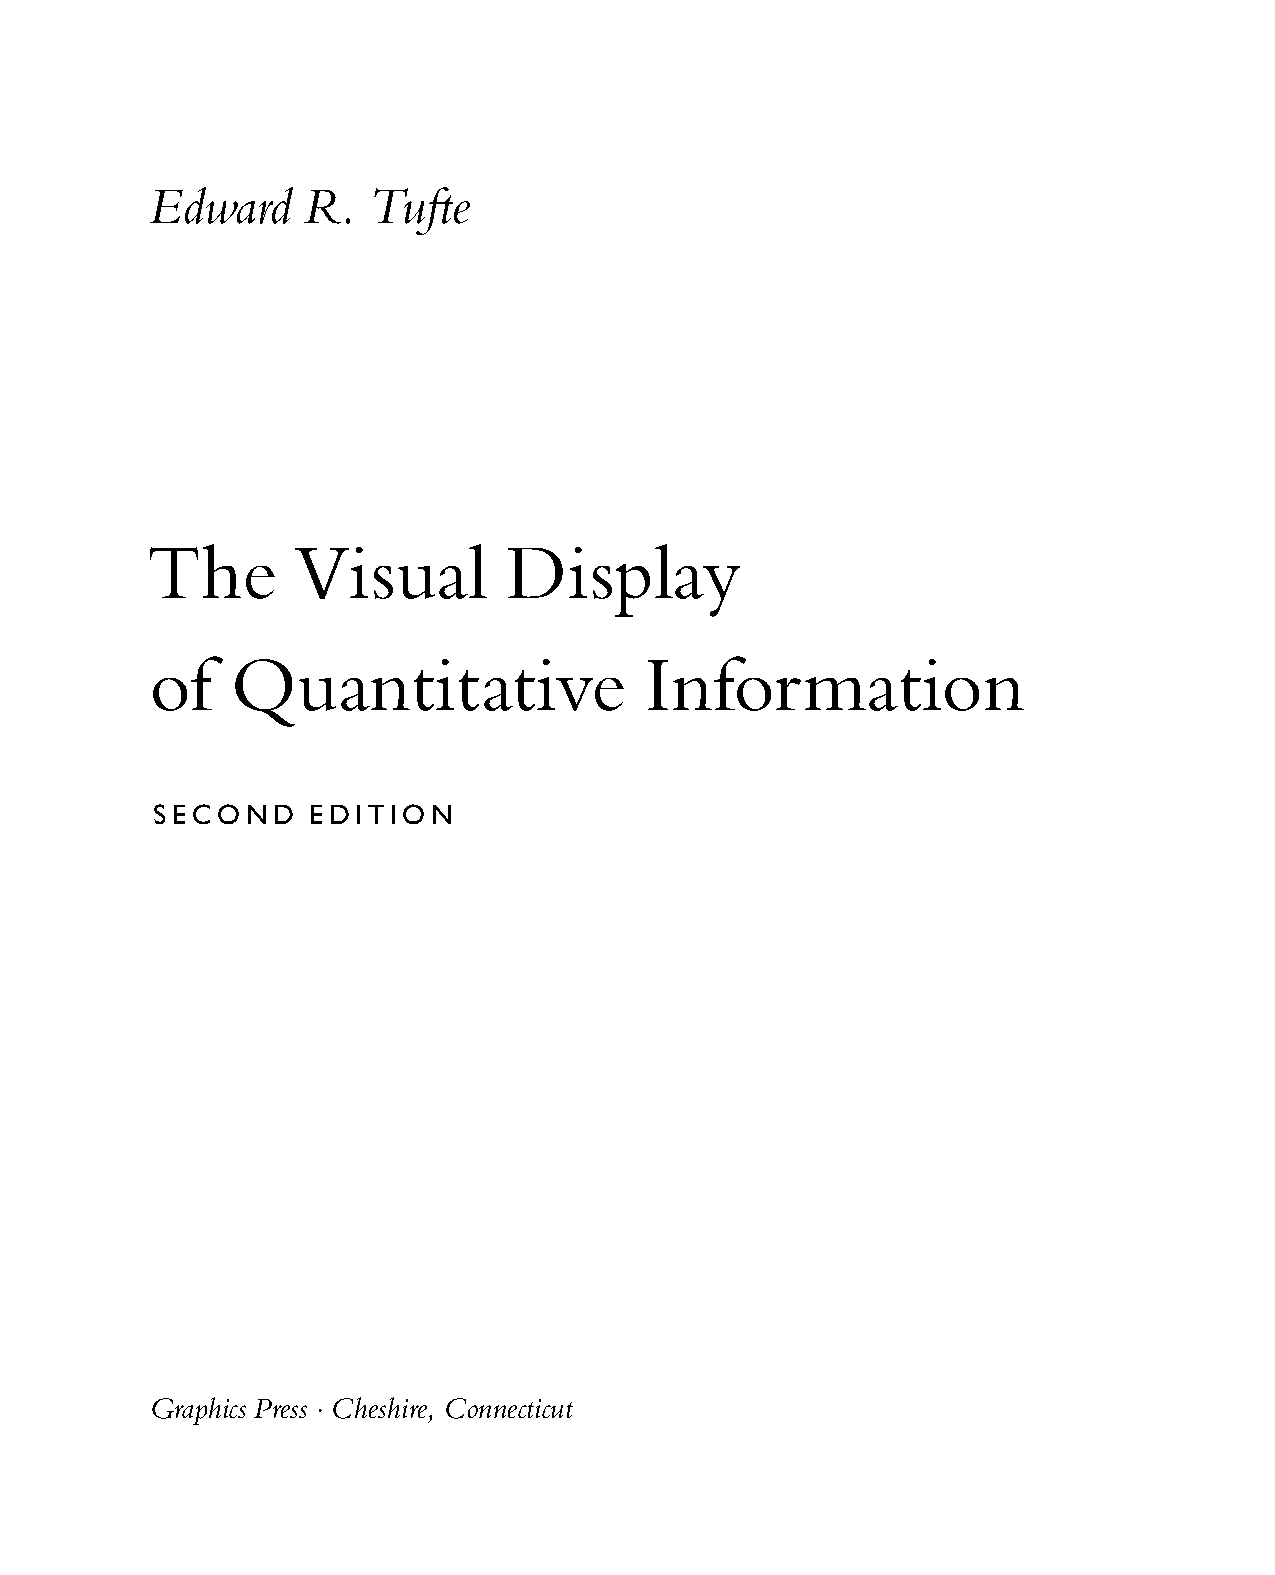
\includegraphics[width=0.45\linewidth]{template/vdqi-title.pdf}}
\hfill
\fbox{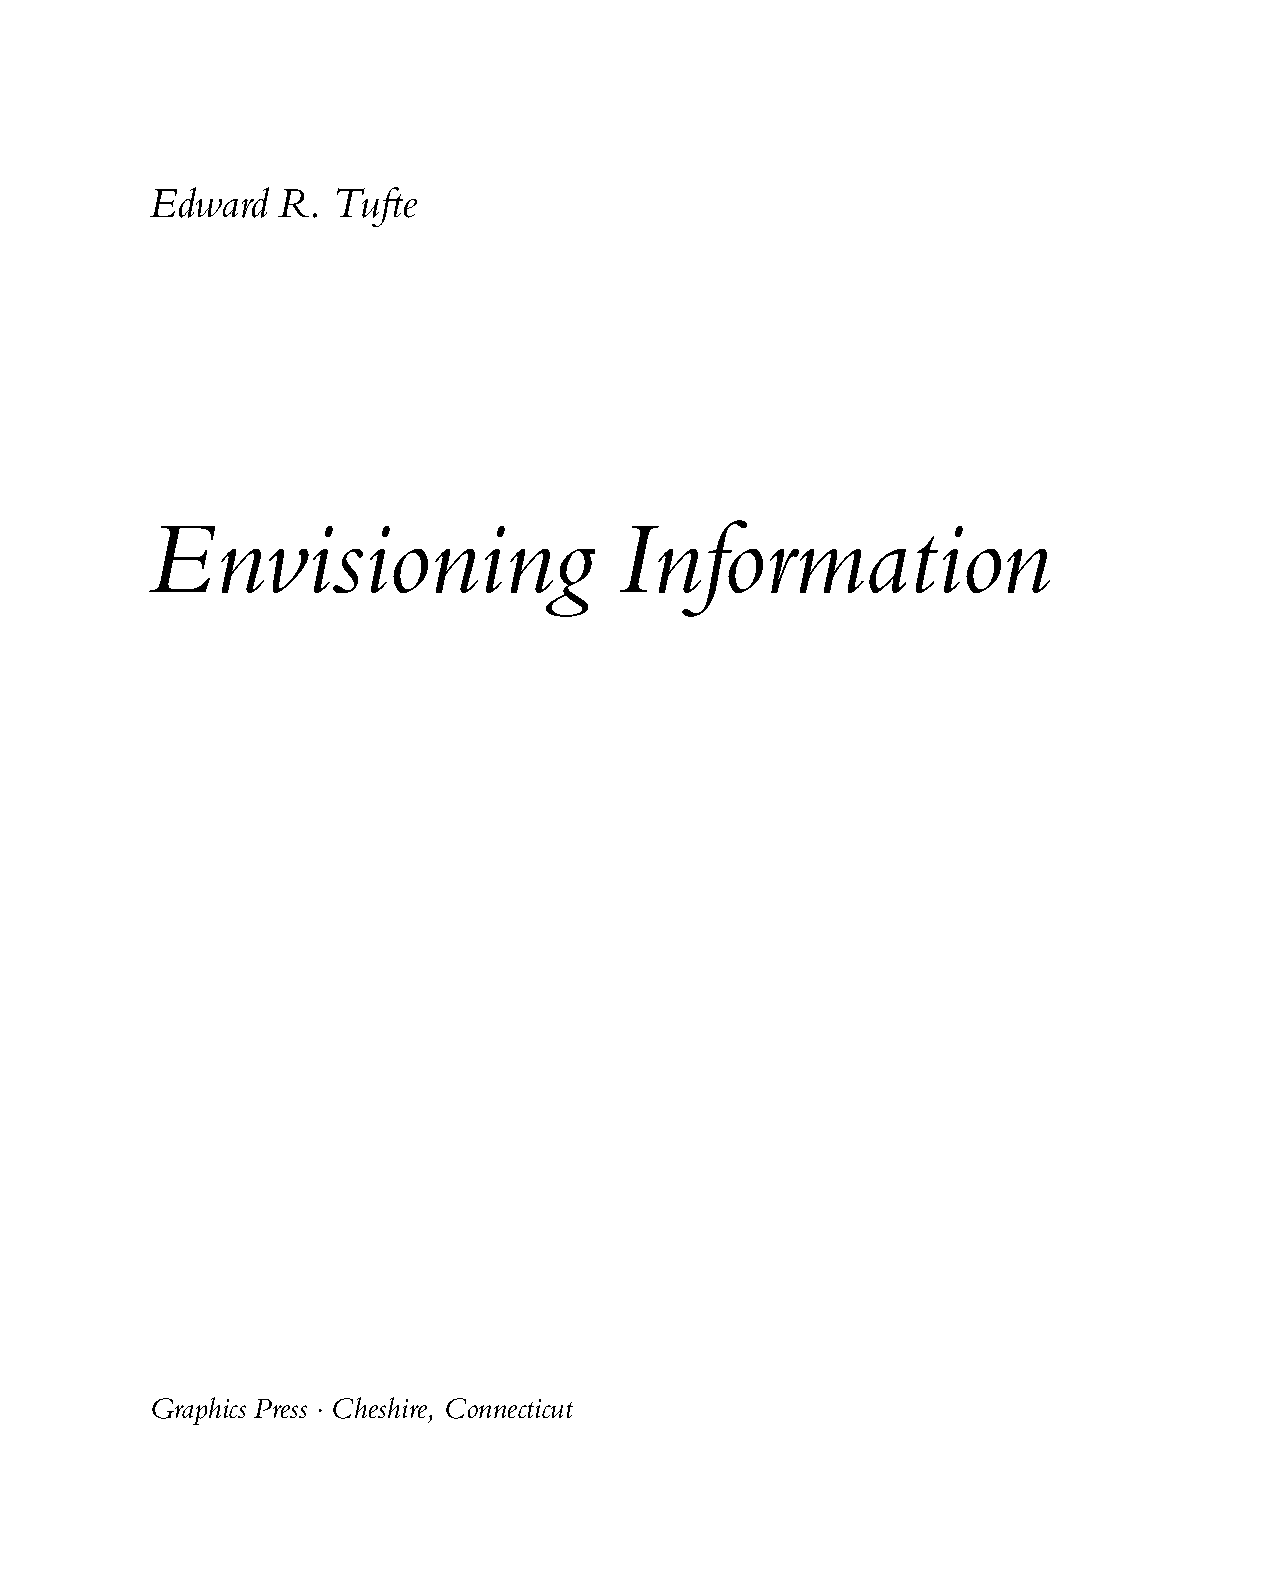
\includegraphics[width=0.45\linewidth]{template/ei-title.pdf}}
\\\vspace{\baselineskip}
\fbox{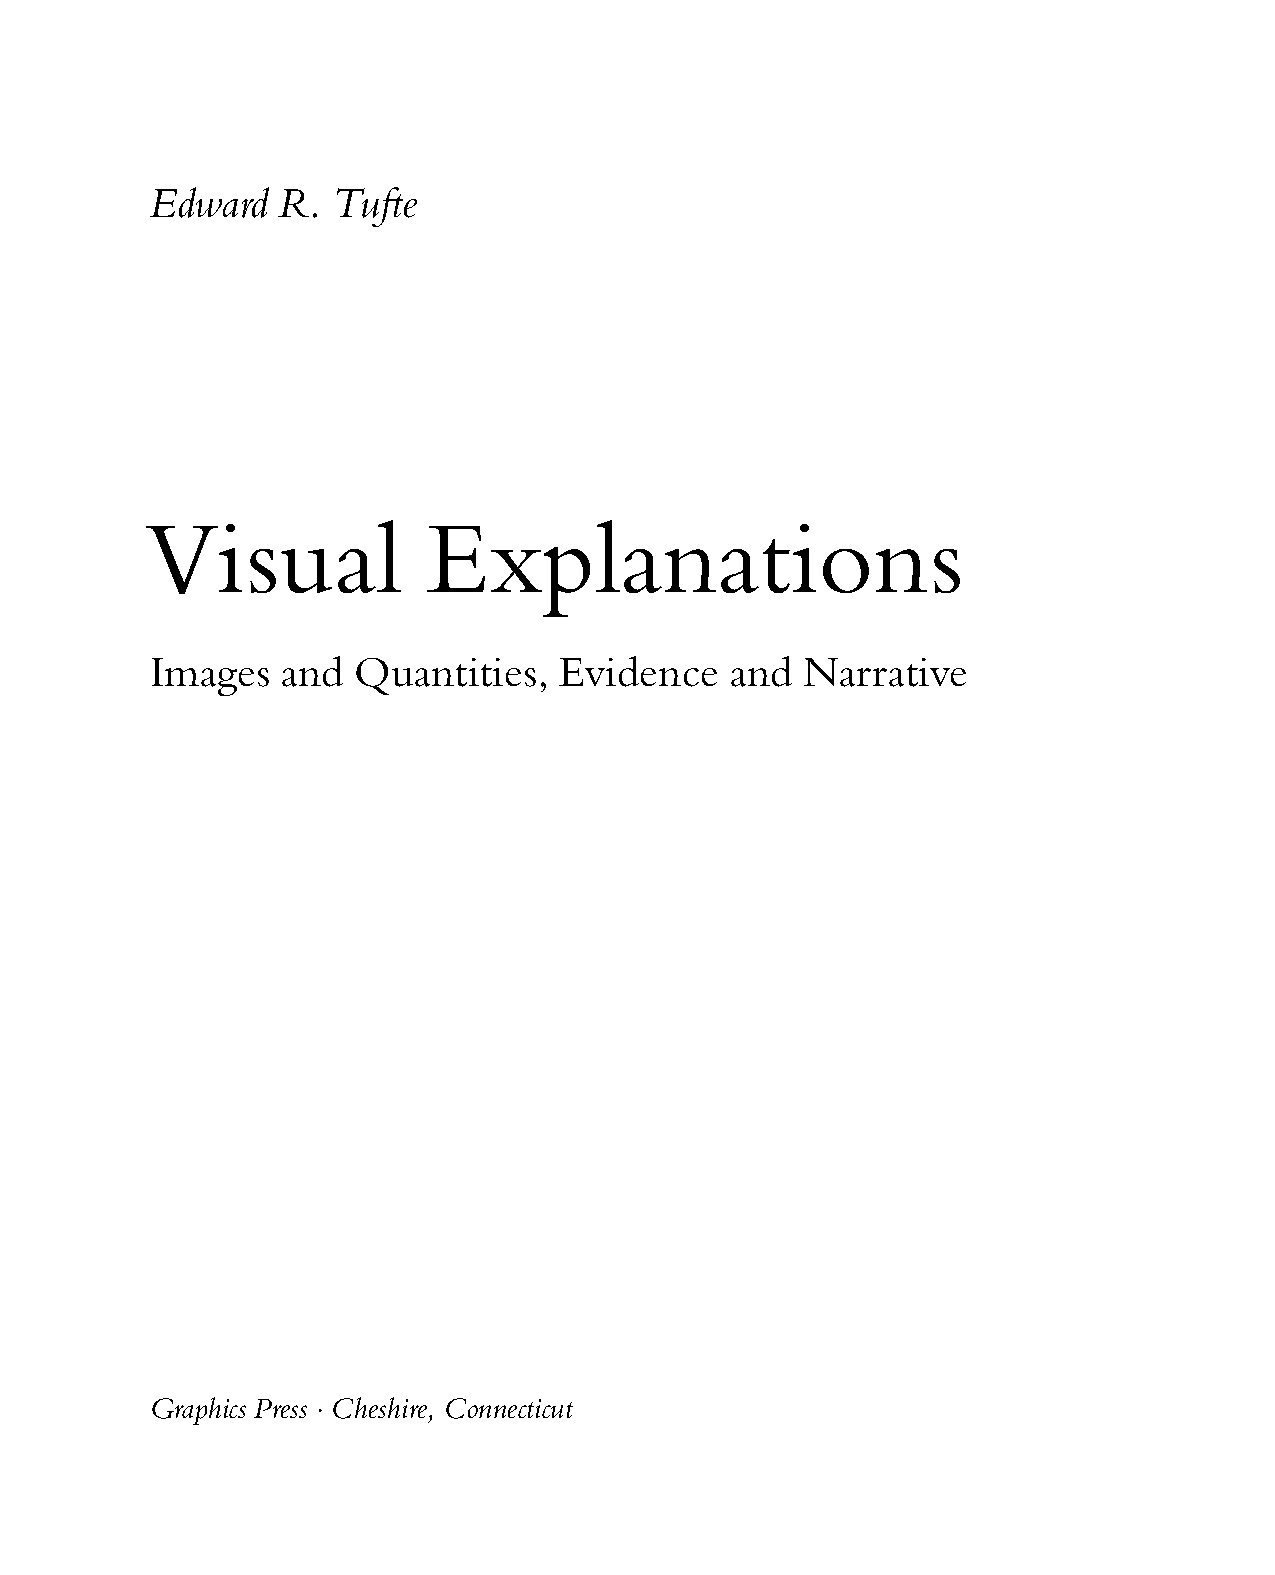
\includegraphics[width=0.45\linewidth]{template/ve-title.pdf}}
\hfill
\fbox{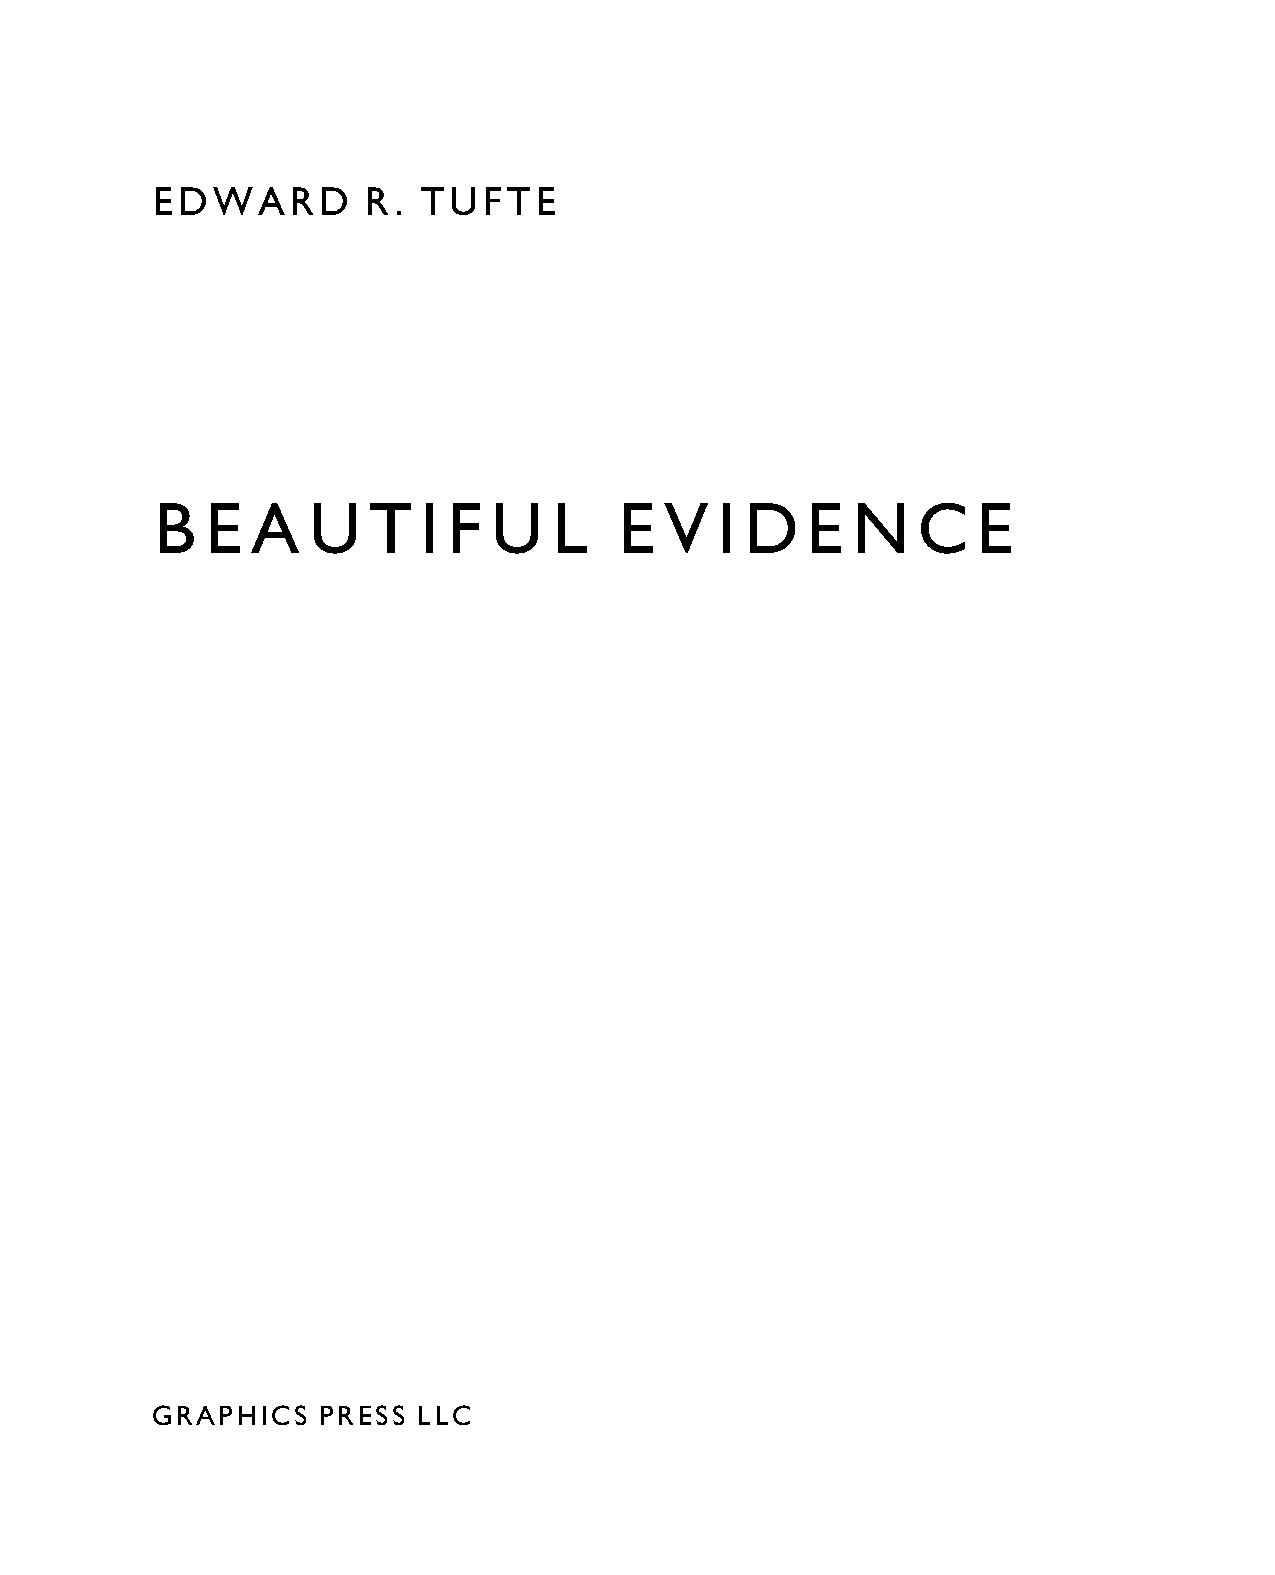
\includegraphics[width=0.45\linewidth]{template/be-title.pdf}}
\end{figure*}

\lipsum[4]
\par\endgroup
% END TUFTE PLACEHOLDER


% !TEX root = ../../../main.tex
\chapter{Metric spaces and topology}
\label{ch:analysis-i:metric-spaces-and-topology}

% !TEX root = ../../../main.tex
\section{Metric spaces}
\label{sec:analysis-i:metric-spaces}

% BEGIN TUFTE PLACEHOLDER: supplied sample, lines 431--446.
\begingroup\sloppy
% Replace this entire specimen block with reviewed course notes.
\newthought{The tables of contents} in Tufte's books give us our first
glimpse of the structure of the main matter.  \VDQI is split into two
parts, each containing some number of chapters.  His other three books only
contain chapters---they're not broken into parts.

\begin{figure*}[p]\index{table of contents}
\fbox{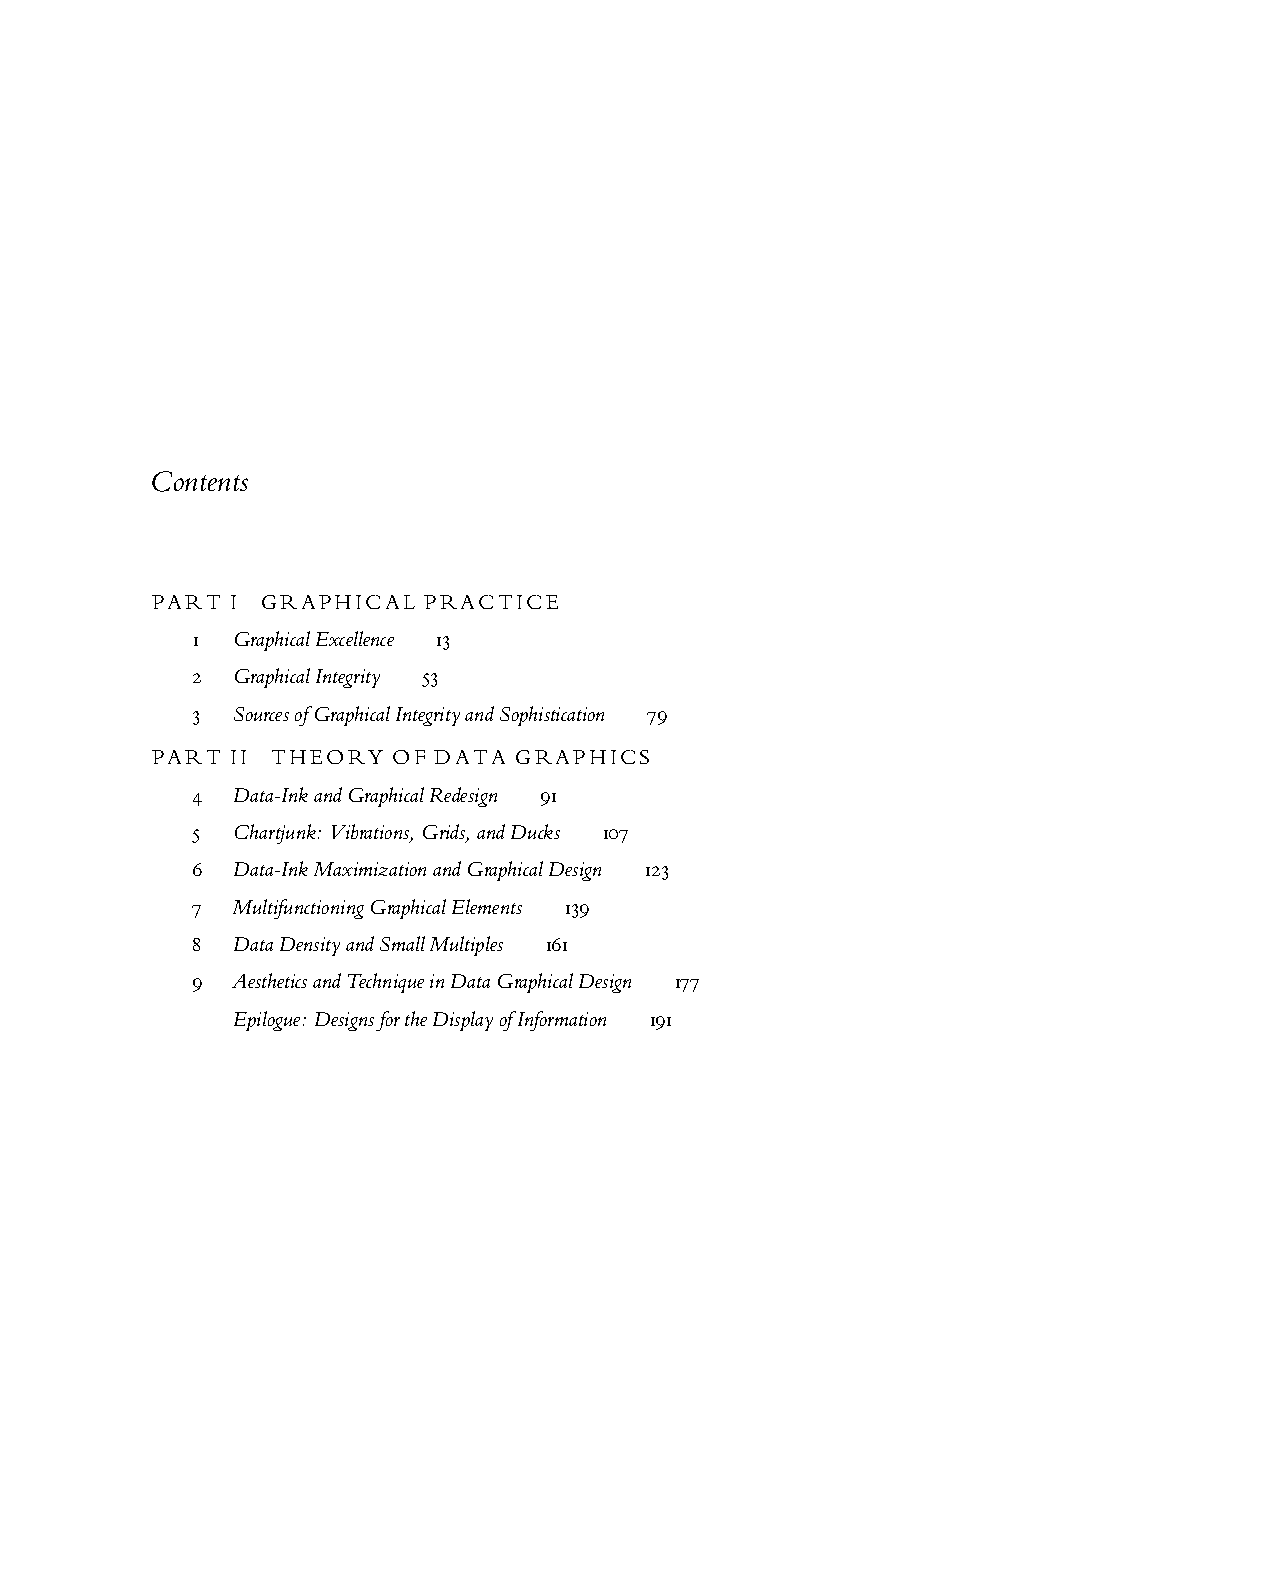
\includegraphics[width=0.45\linewidth]{template/vdqi-contents.pdf}}
\hfill
\fbox{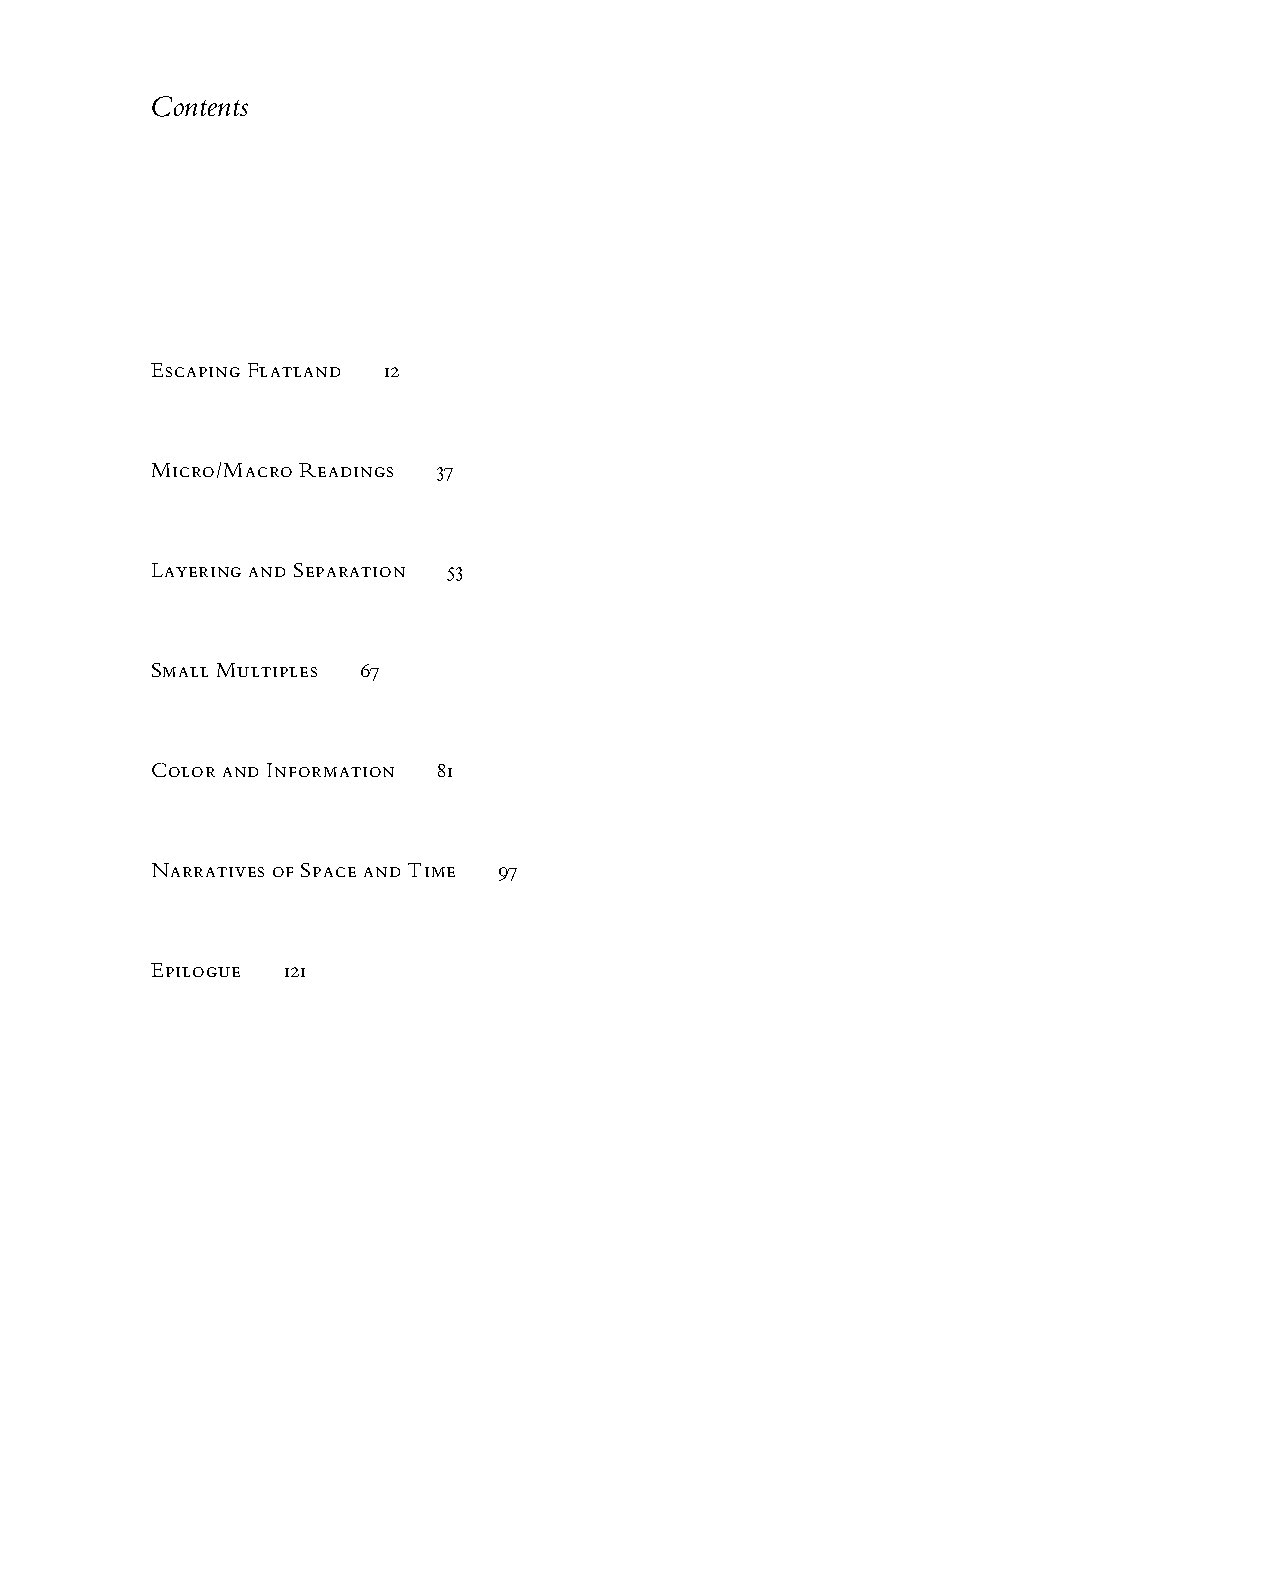
\includegraphics[width=0.45\linewidth]{template/ei-contents.pdf}}
\\\vspace{\baselineskip}
\fbox{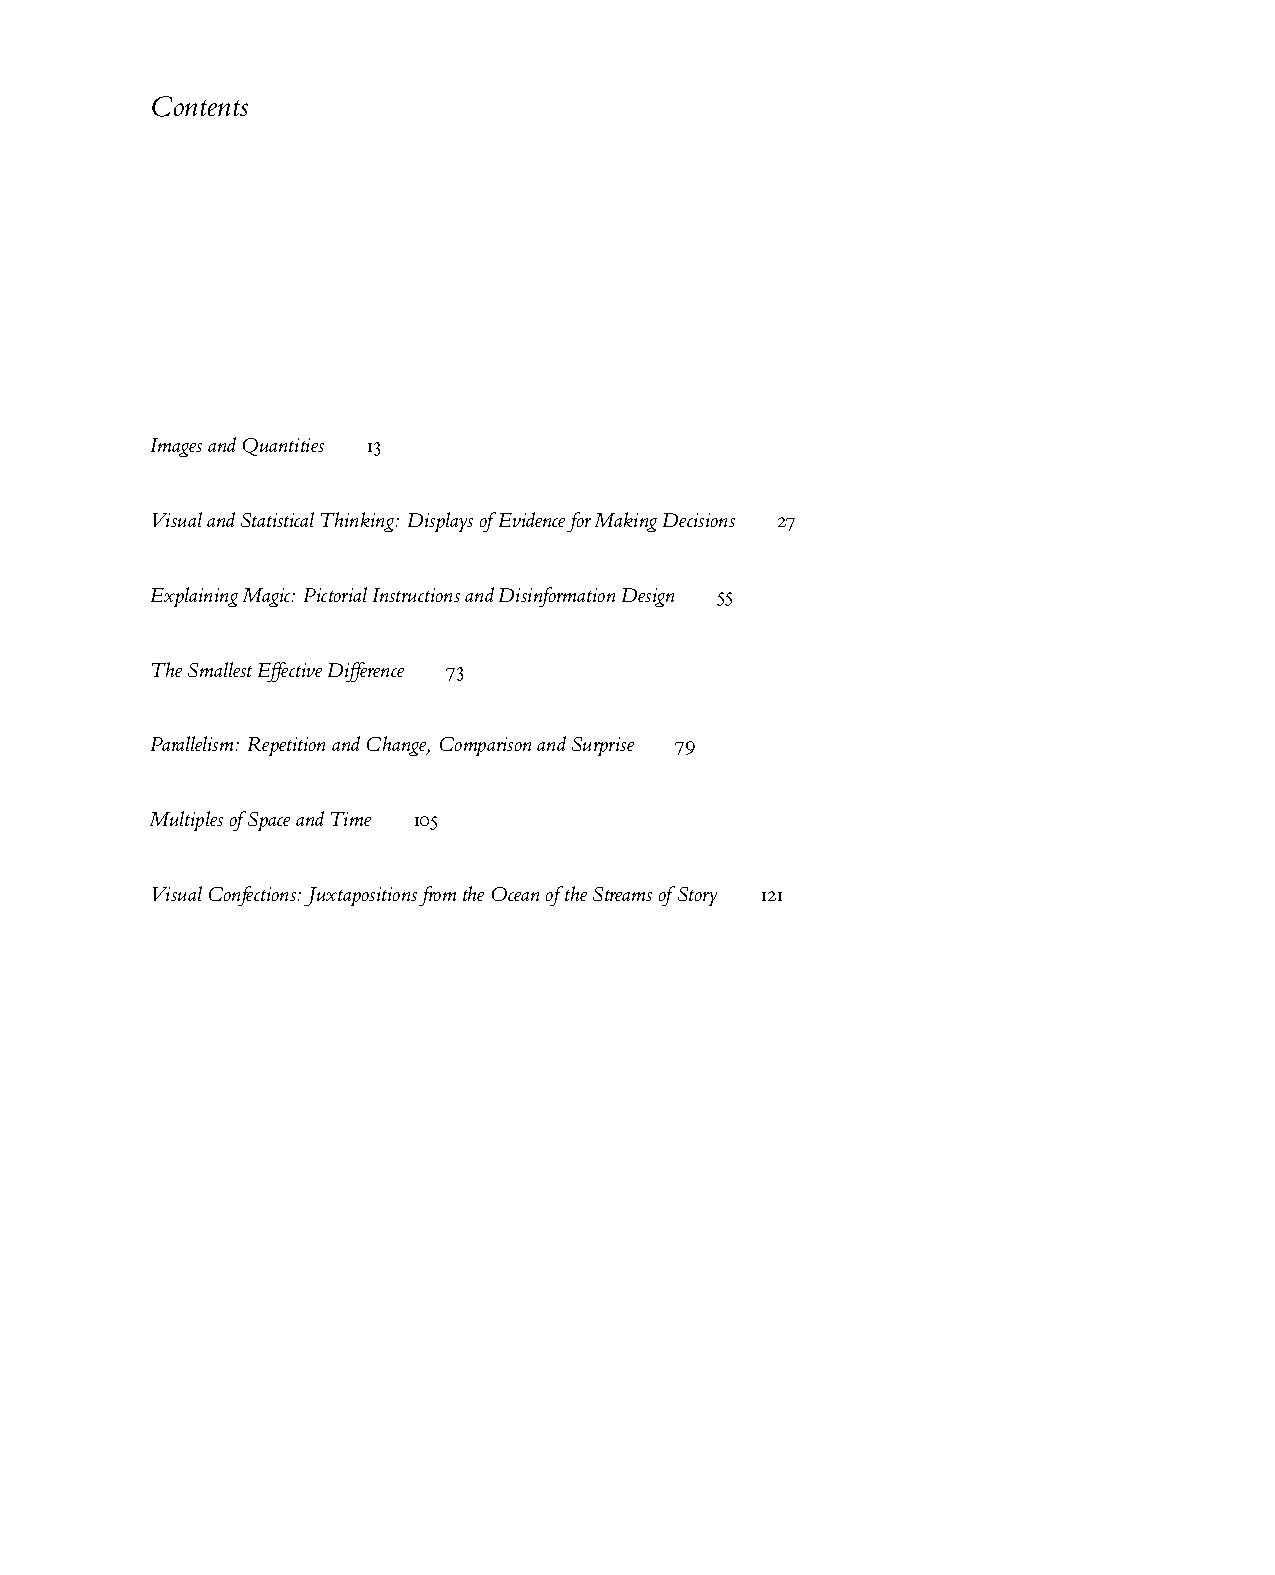
\includegraphics[width=0.45\linewidth]{template/ve-contents.pdf}}
\hfill
\fbox{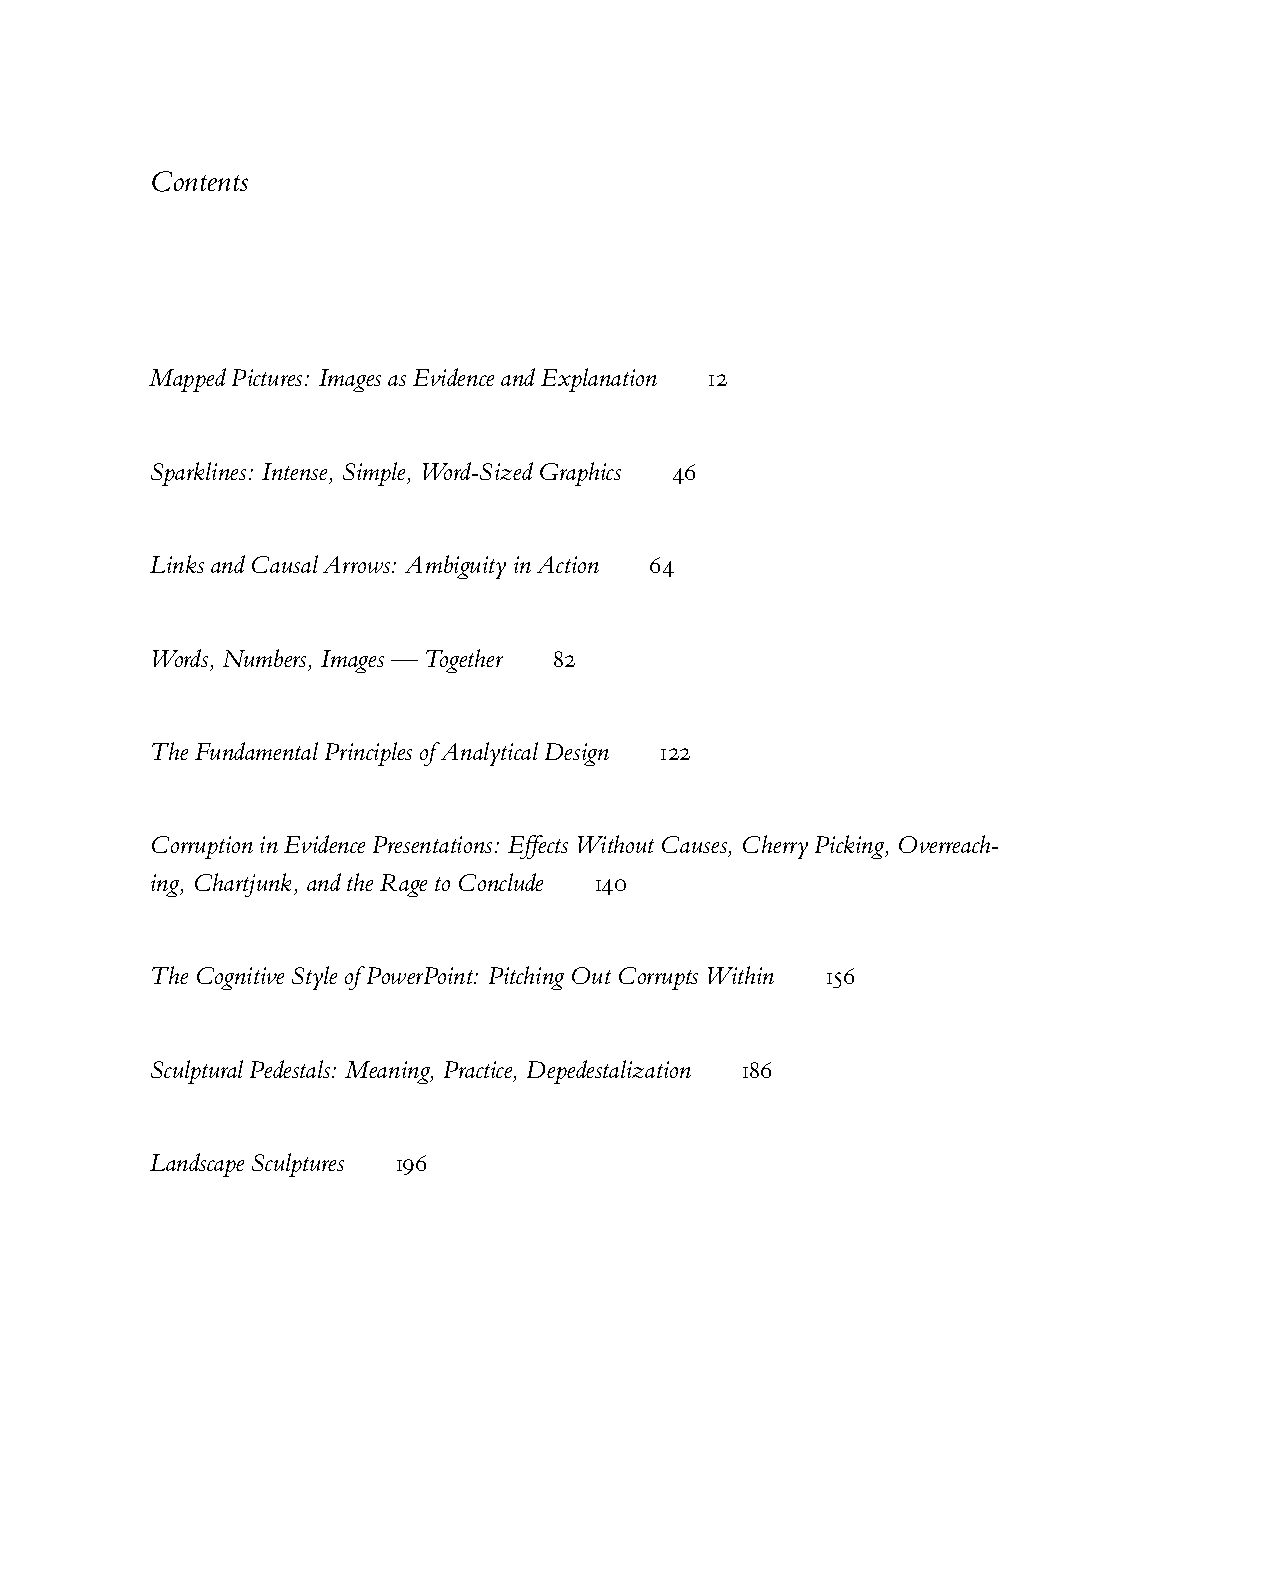
\includegraphics[width=0.45\linewidth]{template/be-contents.pdf}}
\end{figure*}

\lipsum[2]
\par\endgroup
% END TUFTE PLACEHOLDER

% !TEX root = ../../../main.tex
\section{Open, closed, and compact sets}
\label{sec:analysis-i:open-closed-and-compact-sets}

% BEGIN TUFTE PLACEHOLDER: supplied sample, lines 447--484.
\begingroup\sloppy
% Replace this entire specimen block with reviewed course notes.
\label{template:sec:typefaces1}\index{typefaces}
\index{fonts|see{typefaces}}

Tufte's books primarily use two typefaces: Bembo and Gill Sans.  Bembo is used
for the headings and body text, while Gill Sans is used for the title page and
opening epigraphs in \BE.

Since neither Bembo nor Gill Sans are available in default \LaTeX{}
installations, the \TL document classes default to using Palatino and
Helvetica, respectively.  In addition, the Bera Mono typeface is used for
\texttt{monospaced} type.

The following font sizes are defined by the \TL classes:

\begin{table}[h]\index{typefaces!sizes}
  \footnotesize%
  \begin{center}
    \begin{tabular}{lccl}
      \toprule
      \LaTeX{} size & Font size & Leading & Used for \\
      \midrule
      \verb+\tiny+         &  5 &  6 & sidenote numbers \\
      \verb+\scriptsize+   &  7 &  8 & \na \\
      \verb+\footnotesize+ &  8 & 10 & sidenotes, captions \\
      \verb+\small+        &  9 & 12 & quote, quotation, and verse environments \\
      \verb+\normalsize+   & 10 & 14 & body text \\
      \verb+\large+        & 11 & 15 & \textsc{b}-heads \\
      \verb+\Large+        & 12 & 16 & \textsc{a}-heads, \textsc{toc} entries, author, date \\
      \verb+\LARGE+        & 14 & 18 & handout title \\
      \verb+\huge+         & 20 & 30 & chapter heads \\
      \verb+\Huge+         & 24 & 36 & part titles \\
      \bottomrule
    \end{tabular}
  \end{center}
  \caption[Font sizes.]{A list of \LaTeX{} font sizes as defined by the \TL document classes.}
  \label{template:tab:font-sizes}
\end{table}

\lipsum[3]
\par\endgroup
% END TUFTE PLACEHOLDER

% !TEX root = ../../../main.tex
\section{Limit points}
\label{sec:analysis-i:limit-points}

% BEGIN TUFTE PLACEHOLDER: supplied sample, lines 485--513.
\begingroup\sloppy
% Replace this entire specimen block with reviewed course notes.
\label{template:sec:headings1}\index{headings}

Tufte's books include the following heading levels: parts,
chapters,\sidenote{Parts and chapters are defined for the \texttt{tufte-book}
class only.}  sections, subsections, and paragraphs.  Not defined by default
are: sub-subsections and subparagraphs.

\begin{table}[h]
  \begin{center}
    \footnotesize%
    \begin{tabular}{lcr}
      \toprule
      Heading & Style & Size \\
      \midrule
      Part & roman & \measure{24}{36}{40} \\
      Chapter & italic & \measure{20}{30}{40} \\
      Section & italic & \measure{12}{16}{26} \\
      Subsection & italic & \measure{11}{15}{26} \\
      Paragraph & italic & 10/14 \\
      \bottomrule
    \end{tabular}
  \end{center}
  \caption{Heading styles used in \BE.}
  \label{template:tab:heading-styles}
\end{table}

\paragraph{Paragraph} Paragraph headings (as shown here) are introduced by
italicized text and separated from the main paragraph by a bit of space.

\lipsum[4]
\par\endgroup
% END TUFTE PLACEHOLDER

% !TEX root = ../../../main.tex
\section{Heine--Borel theorem}
\label{sec:analysis-i:heine-borel-theorem}

% BEGIN TUFTE PLACEHOLDER: supplied sample, lines 514--537.
\begingroup\sloppy
% Replace this entire specimen block with reviewed course notes.
The following characteristics define the various environments:


\begin{table}[h]
  \begin{center}
    \footnotesize%
    \begin{tabular}{lc p{0.48\linewidth}}
      \toprule
      Environment & Font size & Notes \\
      \midrule
      Body text & \measure{10}{14}{26} & \\
      Block quote & \measure{9}{12}{24} & Block indent (left and right) by \unit[1]{pc} \\
      Sidenotes & \measure{8}{10}{12} & Sidenote number is set inline, followed by word space \\
      Captions & \measure{8}{10}{12} &  \\
      \bottomrule
    \end{tabular}
  \end{center}
  \caption{Environment styles used in \BE.}
  \label{template:tab:environment-styles}
\end{table}

\lipsum[5]
\par\endgroup
% END TUFTE PLACEHOLDER


% !TEX root = ../../../main.tex
\chapter{Sequences of real numbers}
\label{ch:analysis-i:sequences-of-real-numbers}

% !TEX root = ../../../main.tex
\section{Convergent sequences}
\label{sec:analysis-i:convergent-sequences}

% BEGIN TUFTE PLACEHOLDER: supplied sample, lines 538--547.
\begingroup\sloppy
% Replace this entire specimen block with reviewed course notes.
\label{template:ch:tufte-book}

The \TL document classes define a style similar to the
style Edward Tufte uses in his books and handouts.  Tufte's style is known
for its extensive use of sidenotes, tight integration of graphics with
text, and well-set typography.  This document aims to be at once a
demonstration of the features of the \TL document classes
and a style guide to their use.

\lipsum[3]
\par\endgroup
% END TUFTE PLACEHOLDER

% !TEX root = ../../../main.tex
\section{Monotone bounded sequence theorem}
\label{sec:analysis-i:monotone-bounded-sequence-theorem}

% BEGIN TUFTE PLACEHOLDER: supplied sample, lines 548--571.
\begingroup\sloppy
% Replace this entire specimen block with reviewed course notes.
\label{template:sec:page-layout}
\label{template:sec:headings}\index{headings}
This style provides \textsc{a}- and \textsc{b}-heads (that is,
\Verb|\section| and \Verb|\subsection|), demonstrated above.

If you need more than two levels of section headings, you'll have to define
them yourself at the moment; there are no pre-defined styles for anything below
a \Verb|\subsection|.  As Bringhurst points out in \textit{The Elements of
Typographic Style},\cite{Bringhurst2005} you should ``use as many levels of
headings as you need: no more, and no fewer.''

The \TL classes will emit an error if you try to use
\linebreak\Verb|\subsubsection| and smaller headings.

% let's start a new thought -- a new section
\newthought{In his later books},\cite{Tufte2006} Tufte
starts each section with a bit of vertical space, a non-indented paragraph,
and sets the first few words of the sentence in \textsc{small caps}.  To
accomplish this using this style, use the \doccmddef{newthought} command:
\begin{docspec}
  \doccmd{newthought}\{In his later books\}, Tufte starts\ldots
\end{docspec}

\lipsum[4]
\par\endgroup
% END TUFTE PLACEHOLDER

% !TEX root = ../../../main.tex
\section{Bolzano--Weierstrass theorem}
\label{sec:analysis-i:bolzano-weierstrass-theorem}

% BEGIN TUFTE PLACEHOLDER: supplied sample, lines 572--602.
\begingroup\sloppy
% Replace this entire specimen block with reviewed course notes.
\label{template:sec:sidenotes}
One of the most prominent and distinctive features of this style is the
extensive use of sidenotes.  There is a wide margin to provide ample room
for sidenotes and small figures.  Any \doccmd{footnote}s will automatically
be converted to sidenotes.\footnote{This is a sidenote that was entered
using the \texttt{\textbackslash footnote} command.}  If you'd like to place ancillary
information in the margin without the sidenote mark (the superscript
number), you can use the \doccmd{marginnote} command.\marginnote{This is a
margin note.  Notice that there isn't a number preceding the note, and
there is no number in the main text where this note was written.}

The specification of the \doccmddef{sidenote} command is:
\begin{docspec}
  \doccmd{sidenote}[\docopt{number}][\docopt{offset}]\{\docarg{Sidenote text.}\}
\end{docspec}

Both the \docopt{number} and \docopt{offset} arguments are optional.  If you
provide a \docopt{number} argument, then that number will be used as the
sidenote number.  It will change of the number of the current sidenote only and
will not affect the numbering sequence of subsequent sidenotes.

Sometimes a sidenote may run over the top of other text or graphics in the
margin space.  If this happens, you can adjust the vertical position of the
sidenote by providing a dimension in the \docopt{offset} argument.  Some
examples of valid dimensions are:
\begin{docspec}
  \ttfamily 1.0in \qquad 2.54cm \qquad 254mm \qquad 6\Verb|\baselineskip|
\end{docspec}
If the dimension is positive it will push the sidenote down the page; if the
dimension is negative, it will move the sidenote up the page.

\lipsum[5]
\par\endgroup
% END TUFTE PLACEHOLDER

% !TEX root = ../../../main.tex
\section{Upper and lower limits (lim sup and lim inf)}
\label{sec:analysis-i:upper-and-lower-limits}

% BEGIN TUFTE PLACEHOLDER: supplied sample, lines 603--622.
\begingroup\sloppy
% Replace this entire specimen block with reviewed course notes.
While both the \docopt{number} and \docopt{offset} arguments are optional, they
must be provided in order.  To adjust the vertical position of the sidenote
while leaving the sidenote number alone, use the following syntax:
\begin{docspec}
  \doccmd{sidenote}[][\docopt{offset}]\{\docarg{Sidenote text.}\}
\end{docspec}
The empty brackets tell the \Verb|\sidenote| command to use the default
sidenote number.

If you \emph{only} want to change the sidenote number, however, you may
completely omit the \docopt{offset} argument:
\begin{docspec}
  \doccmd{sidenote}[\docopt{number}]\{\docarg{Sidenote text.}\}
\end{docspec}

The \doccmddef{marginnote} command has a similar \docarg{offset} argument:
\begin{docspec}
  \doccmd{marginnote}[\docopt{offset}]\{\docarg{Margin note text.}\}
\end{docspec}

\lipsum[6]
\par\endgroup
% END TUFTE PLACEHOLDER

% !TEX root = ../../../main.tex
\section{Cauchy sequences}
\label{sec:analysis-i:cauchy-sequences}

% BEGIN TUFTE PLACEHOLDER: supplied sample, lines 623--639.
\begingroup\sloppy
% Replace this entire specimen block with reviewed course notes.
References are placed alongside their citations as sidenotes,
as well.  This can be accomplished using the normal \doccmddef{cite}
command.\sidenote{The first paragraph of this document includes a citation.}

The complete list of references may also be printed automatically by using
the \doccmddef{bibliography} command.  (See the end of this document for an
example.)  If you do not want to print a bibliographyn at the end of your
document, use the \doccmddef{nobibliography} command in its place.  

To enter multiple citations at one location,\cite[-3\baselineskip]{Tufte2006,Tufte1990} you can
provide a list of keys separated by commas and the same optional vertical
offset argument: \Verb|\cite{Tufte2006,Tufte1990}|.  
\begin{docspec}
  \doccmd{cite}[\docopt{offset}]\{\docarg{bibkey1,bibkey2,\ldots}\}
\end{docspec}

\lipsum[7]
\par\endgroup
% END TUFTE PLACEHOLDER


% !TEX root = ../../../main.tex
\chapter{Infinite series of numbers}
\label{ch:analysis-i:infinite-series-of-numbers}

% !TEX root = ../../../main.tex
\section{Number series}
\label{sec:analysis-i:number-series}

% BEGIN TUFTE PLACEHOLDER: supplied sample, lines 640--677.
\begingroup\sloppy
% Replace this entire specimen block with reviewed course notes.
\label{template:sec:figures-and-tables}
Images and graphics play an integral role in Tufte's work.
In addition to the standard \docenvdef{figure} and \docenvdef{tabular} environments,
this style provides special figure and table environments for full-width
floats.

Full page--width figures and tables may be placed in \docenvdef{figure*} or
\docenvdef{table*} environments.  To place figures or tables in the margin,
use the \docenvdef{marginfigure} or \docenvdef{margintable} environments as follows
(see figure~\ref{template:fig:marginfig}):

\begin{marginfigure}%
  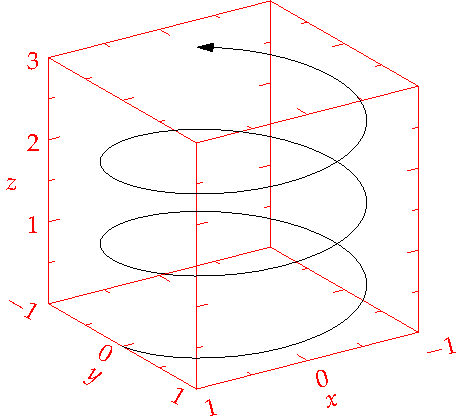
\includegraphics[width=\linewidth]{template/helix}
  \caption[Helix in the margin.]{This is a margin figure.  The helix is defined by 
    $x = \cos(2\pi z)$, $y = \sin(2\pi z)$, and $z = [0, 2.7]$.  The figure was
    drawn using Asymptote (\protect\url{http://asymptote.sf.net/}).}
  \label{template:fig:marginfig}
\end{marginfigure}

\begin{docspec}
\textbackslash begin\{marginfigure\}\\
  \qquad\textbackslash includegraphics\{helix\}\\
  \qquad\textbackslash caption\{This is a margin figure.\}\\
  \qquad\textbackslash label\{fig:marginfig\}\\
\textbackslash end\{marginfigure\}\\
\end{docspec}

The \docenv{marginfigure} and \docenv{margintable} environments accept an optional parameter \docopt{offset} that adjusts the vertical position of the figure or table.  See the ``\nameref{template:sec:sidenotes}'' section above for examples.  The specifications are:
\begin{docspec}
  \textbackslash{begin\{marginfigure\}[\docopt{offset}]}\\
  \qquad\ldots\\
  \textbackslash{end\{marginfigure\}}\\
  \mbox{}\\
  \textbackslash{begin\{margintable\}[\docopt{offset}]}\\
  \qquad\ldots\\
  \textbackslash{end\{margintable\}}\\
\end{docspec}

\lipsum[4]
\par\endgroup
% END TUFTE PLACEHOLDER

% !TEX root = ../../../main.tex
\section{Comparison tests}
\label{sec:analysis-i:comparison-tests}

% BEGIN TUFTE PLACEHOLDER: supplied sample, lines 678--688.
\begingroup\sloppy
% Replace this entire specimen block with reviewed course notes.
Figure~\ref{template:fig:fullfig} is an example of the \docenv{figure*}
environment and figure~\ref{template:fig:textfig} is an example of the normal
\docenv{figure} environment.

\begin{figure*}[h]
  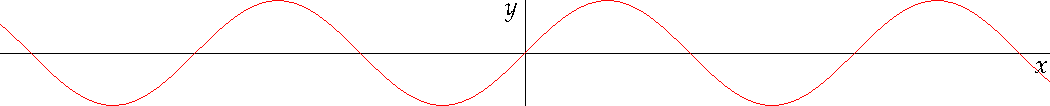
\includegraphics[width=\linewidth]{template/sine.pdf}%
  \caption[Full-width sine wave.]{This graph shows $y = \sin x$ from about $x = [-10, 10]$.
  \emph{Notice that this figure takes up the full page width.}}%
  \label{template:fig:fullfig}%
\end{figure*}

\lipsum[5]
\par\endgroup
% END TUFTE PLACEHOLDER

% !TEX root = ../../../main.tex
\section{Dirichlet test}
\label{sec:analysis-i:dirichlet-test}

% BEGIN TUFTE PLACEHOLDER: supplied sample, lines 689--696.
\begingroup\sloppy
% Replace this entire specimen block with reviewed course notes.
\begin{figure}
  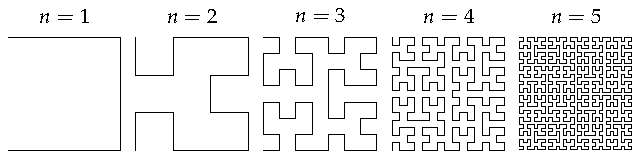
\includegraphics{template/hilbertcurves.pdf}
%  \checkparity This is an \pageparity\ page.%
  \caption[Hilbert curves of various degrees $n$.][6pt]{Hilbert curves of various degrees $n$. \emph{Notice that this figure only takes up the main textblock width.}}
  \label{template:fig:textfig}
  %\zsavepos{pos:textfig}
\end{figure}

\lipsum[6]
\par\endgroup
% END TUFTE PLACEHOLDER

% !TEX root = ../../../main.tex
\section{Conditional convergence}
\label{sec:analysis-i:conditional-convergence}

% BEGIN TUFTE PLACEHOLDER: supplied sample, lines 697--719.
\begingroup\sloppy
% Replace this entire specimen block with reviewed course notes.
As with sidenotes and marginnotes, a caption may sometimes require vertical
adjustment. The \doccmddef{caption} command now takes a second optional
argument that enables you to do this by providing a dimension \docopt{offset}.
You may specify the caption in any one of the following forms:
\begin{docspec}
  \doccmd{caption}\{\docarg{long caption}\}\\
  \doccmd{caption}[\docarg{short caption}]\{\docarg{long caption}\}\\
  \doccmd{caption}[][\docopt{offset}]\{\docarg{long caption}\}\\
  \doccmd{caption}[\docarg{short caption}][\docopt{offset}]%
                  \{\docarg{long caption}\}
\end{docspec}
A positive \docopt{offset} will push the caption down the page. The short
caption, if provided, is what appears in the list of figures/tables, otherwise
the ``long'' caption appears there. Note that although the arguments
\docopt{short caption} and \docopt{offset} are both optional, they must be
provided in order. Thus, to specify an \docopt{offset} without specifying a
\docopt{short caption}, you must include the first set of empty brackets
\Verb|[]|, which tell \doccmd{caption} to use the default ``long'' caption. As
an example, the caption to figure~\ref{template:fig:textfig} above was given in the form
\begin{docspec}
  \doccmd{caption}[Hilbert curves...][6pt]\{Hilbert curves...\}
\end{docspec}

\lipsum[7]
\par\endgroup
% END TUFTE PLACEHOLDER


% !TEX root = ../../../main.tex
\chapter{Continuity}
\label{ch:analysis-i:continuity}

% !TEX root = ../../../main.tex
\section{Continuity}
\label{sec:analysis-i:continuity}

% BEGIN TUFTE PLACEHOLDER: supplied sample, lines 720--742.
\begingroup\sloppy
% Replace this entire specimen block with reviewed course notes.
Table~\ref{template:tab:normaltab} shows table created with the \docpkg{booktabs}
package.  Notice the lack of vertical rules---they serve only to clutter
the table's data.

\begin{table}[ht]
  \centering
  \fontfamily{ppl}\selectfont
  \begin{tabular}{ll}
    \toprule
    Margin & Length \\
    \midrule
    Paper width & \unit[8\nicefrac{1}{2}]{inches} \\
    Paper height & \unit[11]{inches} \\
    Textblock width & \unit[6\nicefrac{1}{2}]{inches} \\
    Textblock/sidenote gutter & \unit[\nicefrac{3}{8}]{inches} \\
    Sidenote width & \unit[2]{inches} \\
    \bottomrule
  \end{tabular}
  \caption[Page dimensions.]{Here are the dimensions of the various margins used in the Tufte-handout class.}
  \label{template:tab:normaltab}
  %\zsavepos{pos:normaltab}
\end{table}

\lipsum[5]
\par\endgroup
% END TUFTE PLACEHOLDER

% !TEX root = ../../../main.tex
\section{Maximum (extreme value theorem)}
\label{sec:analysis-i:extreme-value-theorem}

% BEGIN TUFTE PLACEHOLDER: supplied sample, lines 743--764.
\begingroup\sloppy
% Replace this entire specimen block with reviewed course notes.
\newthought{Occasionally} \LaTeX{} will generate an error message:\label{template:err:too-many-floats}
\begin{docspec}
  Error: Too many unprocessed floats
\end{docspec}
\LaTeX{} tries to place floats in the best position on the page.  Until it's
finished composing the page, however, it won't know where those positions are.
If you have a lot of floats on a page (including sidenotes, margin notes,
figures, tables, etc.), \LaTeX{} may run out of ``slots'' to keep track of them
and will generate the above error.

\LaTeX{} initially allocates 18 slots for storing floats.  To work around this
limitation, the \TL document classes provide a \doccmddef{morefloats} command
that will reserve more slots.

The first time \doccmd{morefloats} is called, it allocates an additional 34
slots.  The second time \doccmd{morefloats} is called, it allocates another 26
slots.

The \doccmd{morefloats} command may only be used two times.  Calling it a
third time will generate an error message.  (This is because we can't safely
allocate many more floats or \LaTeX{} will run out of memory.)

\lipsum[6]
\par\endgroup
% END TUFTE PLACEHOLDER

% !TEX root = ../../../main.tex
\section{Intermediate value theorem}
\label{sec:analysis-i:intermediate-value-theorem}

% BEGIN TUFTE PLACEHOLDER: supplied sample, lines 765--783.
\begingroup\sloppy
% Replace this entire specimen block with reviewed course notes.
If, after using the \doccmd{morefloats} command twice, you continue to get the
\texttt{Too many unprocessed floats} error, there are a couple things you can
do.

The \doccmddef{FloatBarrier} command will immediately process all the floats
before typesetting more material.  Since \doccmd{FloatBarrier} will start a new
paragraph, you should place this command at the beginning or end of a
paragraph.

The \doccmddef{clearpage} command will also process the floats before
continuing, but instead of starting a new paragraph, it will start a new page.

You can also try moving your floats around a bit: move a figure or table to the
next page or reduce the number of sidenotes.  (Each sidenote actually uses
\emph{two} slots.)

After the floats have placed, \LaTeX{} will mark those slots as unused so they
are available for the next page to be composed.

\lipsum[7]
\par\endgroup
% END TUFTE PLACEHOLDER

% !TEX root = ../../../main.tex
\section{Uniform continuity}
\label{sec:analysis-i:uniform-continuity}

% BEGIN TUFTE PLACEHOLDER: supplied sample, lines 784--813.
\begingroup\sloppy
% Replace this entire specimen block with reviewed course notes.
You may notice that the captions are sometimes misaligned.
Due to the way \LaTeX's float mechanism works, we can't know for sure where it
decided to put a float. Therefore, the \TL document classes provide commands to
override the caption position.

\paragraph{Vertical alignment} To override the vertical alignment, use the
\doccmd{setfloatalignment} command inside the float environment.  For
example:

\begin{fullwidth}
\begin{docspec}
  \textbackslash begin\{figure\}[btp]\\
  \qquad \textbackslash includegraphics\{sinewave\}\\
  \qquad \textbackslash caption\{This is an example of a sine wave.\}\\
  \qquad \textbackslash label\{fig:sinewave\}\\
  \qquad \hlred{\textbackslash setfloatalignment\{b\}\% forces caption to be bottom-aligned}\\
  \textbackslash end\{figure\}
\end{docspec}
\end{fullwidth}

\noindent The syntax of the \doccmddef{setfloatalignment} command is:

\begin{docspec}
  \doccmd{setfloatalignment}\{\docopt{pos}\}
\end{docspec}

\noindent where \docopt{pos} can be either \texttt{b} for bottom-aligned
captions, or \texttt{t} for top-aligned captions.

\lipsum[1]
\par\endgroup
% END TUFTE PLACEHOLDER


% !TEX root = ../../../main.tex
\chapter{Differentiation and its applications}
\label{ch:analysis-i:differentiation-and-applications}

% !TEX root = ../../../main.tex
\section{Differentiation}
\label{sec:analysis-i:differentiation}

% BEGIN TUFTE PLACEHOLDER: supplied sample, lines 814--836.
\begingroup\sloppy
% Replace this entire specimen block with reviewed course notes.
\paragraph{Horizontal alignment}\label{template:par:overriding-horizontal}
To override the horizontal alignment, use either the \doccmd{forceversofloat}
or the \doccmd{forcerectofloat} command inside of the float environment.  For
example:

\begin{fullwidth}
\begin{docspec}
  \textbackslash begin\{figure\}[btp]\\
  \qquad \textbackslash includegraphics\{sinewave\}\\
  \qquad \textbackslash caption\{This is an example of a sine wave.\}\\
  \qquad \textbackslash label\{fig:sinewave\}\\
  \qquad \hlred{\textbackslash forceversofloat\% forces caption to be set to the left of the float}\\
  \textbackslash end\{figure\}
\end{docspec}
\end{fullwidth}

The \doccmddef{forceversofloat} command causes the algorithm to assume the
float has been placed on a verso page---that is, a page on the left side of a
two-page spread.  Conversely, the \doccmddef{forcerectofloat} command causes
the algorithm to assume the float has been placed on a recto page---that is, a
page on the right side of a two-page spread.

\lipsum[6]
\par\endgroup
% END TUFTE PLACEHOLDER

% !TEX root = ../../../main.tex
\section{Mean value theorems}
\label{sec:analysis-i:mean-value-theorems}

% BEGIN TUFTE PLACEHOLDER: supplied sample, lines 837--852.
\begingroup\sloppy
% Replace this entire specimen block with reviewed course notes.
In addition to the new float types, there is a \docenvdef{fullwidth}
environment that stretches across the main text block and the sidenotes
area.

\begin{Verbatim}
\begin{fullwidth}
Lorem ipsum dolor sit amet...
\end{fullwidth}
\end{Verbatim}

\begin{fullwidth}
\small\itshape\lipsum[1]
\end{fullwidth}

\lipsum[7]
\par\endgroup
% END TUFTE PLACEHOLDER

% !TEX root = ../../../main.tex
\section{Taylor's theorem}
\label{sec:analysis-i:taylor-theorem}

% BEGIN TUFTE PLACEHOLDER: supplied sample, lines 853--878.
\begingroup\sloppy
% Replace this entire specimen block with reviewed course notes.
\label{template:sec:typography}

\label{template:sec:typefaces}\index{typefaces}
If the Palatino, \textsf{Helvetica}, and \texttt{Bera Mono} typefaces are installed, this style
will use them automatically.  Otherwise, we'll fall back on the Computer Modern
typefaces.

\label{template:sec:letterspacing}
This document class includes two new commands and some improvements on
existing commands for letterspacing.

When setting strings of \allcaps{ALL CAPS} or \smallcaps{small caps}, the
letter\-spacing---that is, the spacing between the letters---should be
increased slightly.\cite[][p.32]{Bringhurst2005} The \doccmddef{allcaps} command has proper letterspacing for
strings of \allcaps{FULL CAPITAL LETTERS}, and the \doccmddef{smallcaps} command
has letterspacing for \smallcaps{small capital letters}.  These commands
will also automatically convert the case of the text to upper- or
lowercase, respectively.

The \doccmddef{textsc} command has also been redefined to include
letterspacing.  The case of the \doccmd{textsc} argument is left as is,
however.  This allows one to use both uppercase and lowercase letters:
\textsc{The Initial Letters Of The Words In This Sentence Are Capitalized.}

\lipsum[1]
\par\endgroup
% END TUFTE PLACEHOLDER

% !TEX root = ../../../main.tex
\section{Convex functions}
\label{sec:analysis-i:convex-functions}

% BEGIN TUFTE PLACEHOLDER: supplied sample, lines 879--907.
\begingroup\sloppy
% Replace this entire specimen block with reviewed course notes.
\label{template:sec:options}

\index{class options|(}
The \doccls{tufte-book} class is based on the \LaTeX\ \doccls{book}
document class.  Therefore, you can pass any of the typical book
options.  There are a few options that are specific to the
\doccls{tufte-book} document class, however.

The \docclsoptdef{a4paper} option will set the paper size to \smallcaps{A4} instead of
the default \smallcaps{US} letter size.

The \docclsoptdef{sfsidenotes} option will set the sidenotes and title block in a 
\textsf{sans serif} typeface instead of the default roman.

The \docclsoptdef{twoside} option will modify the running heads so that the page
number is printed on the outside edge (as opposed to always printing the page
number on the right-side edge in \docclsoptdef{oneside} mode).  

The \docclsoptdef{symmetric} option typesets the sidenotes on the outside edge of
the page.  This is how books are traditionally printed, but is contrary to
Tufte's book design which sets the sidenotes on the right side of the page.
This option implicitly sets the \docclsopt{twoside} option.

The \docclsoptdef{justified} option sets all the text fully justified (flush left
and right).  The default is to set the text ragged right.  
The body text of Tufte's books are set ragged right.  This prevents
needless hyphenation and makes it easier to read the text in the slightly
narrower column.

\lipsum[2]
\par\endgroup
% END TUFTE PLACEHOLDER

% !TEX root = ../../../main.tex
\section{L'H\^opital's rules}
\label{sec:analysis-i:lhopital-rules}

% BEGIN TUFTE PLACEHOLDER: supplied sample, lines 908--934.
\begingroup\sloppy
% Replace this entire specimen block with reviewed course notes.
The \docclsoptdef{bidi} option loads the \docpkg{bidi} package which is used with
\tXeLaTeX\ to typeset bi-directional text.  Since the \docpkg{bidi}
package needs to be loaded before the sidenotes and cite commands are defined,
it can't be loaded in the document preamble.

The \docclsoptdef{debug} option causes the \TL classes to output debug
information to the log file which is useful in troubleshooting bugs.  It will
also cause the graphics to be replaced by outlines.

The \docclsoptdef{nofonts} option prevents the \TL classes from
automatically loading the Palatino and Helvetica typefaces.  You should use
this option if you wish to load your own fonts.  If you're using \tXeLaTeX, this
option is implied (\ie, the Palatino and Helvetica fonts aren't loaded if you
use \tXeLaTeX).  

The \docclsoptdef{nols} option inhibits the letterspacing code.  The \TL\
classes try to load the appropriate letterspacing package (either pdf\TeX's
\docpkg{letterspace} package or the \docpkg{soul} package).  If you're using
\tXeLaTeX\ with \docpkg{fontenc}, however, you should configure your own
letterspacing.  

The \docclsoptdef{notitlepage} option causes \doccmd{maketitle} to generate a title
block instead of a title page.  The \doccls{book} class defaults to a title
page and the \doccls{handout} class defaults to the title block.  There is an
analogous \docclsoptdef{titlepage} option that forces \doccmd{maketitle} to
generate a full title page instead of the title block.

\lipsum[3]
\par\endgroup
% END TUFTE PLACEHOLDER

% !TEX root = ../../../main.tex
\section{Inverse function theorem}
\label{sec:analysis-i:inverse-function-theorem}

% BEGIN TUFTE PLACEHOLDER: supplied sample, lines 935--948.
\begingroup\sloppy
% Replace this entire specimen block with reviewed course notes.
The \docclsoptdef{notoc} option suppresses \TL's custom table of contents
(\textsc{toc}) design.  The current \textsc{toc} design only shows unnumbered
chapter titles; it doesn't show sections or subsections.  The \docclsopt{notoc}
option will revert to \LaTeX's \textsc{toc} design.

The \docclsoptdef{nohyper} option prevents the \docpkg{hyperref} package from
being loaded.  The default is to load the \docpkg{hyperref} package and use the
\doccmd{title} and \doccmd{author} contents as metadata for the generated
\textsc{pdf}.

\index{class options|)}

\lipsum[4]
\par\endgroup
% END TUFTE PLACEHOLDER


% !TEX root = ../../../main.tex
\chapter{Riemann integration}
\label{ch:analysis-i:riemann-integration}

% !TEX root = ../../../main.tex
\section{Integration}
\label{sec:analysis-i:integration}

% BEGIN TUFTE PLACEHOLDER: supplied sample, lines 949--957.
\begingroup\sloppy
% Replace this entire specimen block with reviewed course notes.
\label{template:ch:customizing}

The \TL document classes are designed to closely emulate Tufte's book
design by default.  However, each document is different and you may encounter
situations where the default settings are insufficient.  This chapter explores
many of the ways you can adjust the \TL document classes to better fit
your needs.

\lipsum[7]
\par\endgroup
% END TUFTE PLACEHOLDER

% !TEX root = ../../../main.tex
\section{Upper and lower sums}
\label{sec:analysis-i:upper-and-lower-sums}

% BEGIN TUFTE PLACEHOLDER: supplied sample, lines 958--985.
\begingroup\sloppy
% Replace this entire specimen block with reviewed course notes.
\label{template:sec:filehooks}

\index{file hooks|(}
If you create many documents using the \TL classes, it's easier to
store your customizations in a separate file instead of copying them into the
preamble of each document.  The \TL classes provide three file hooks:
\docfilehook{tufte-common-local.tex}{common}, \docfilehook{tufte-book-local.tex}{book}, and
\docfilehook{tufte-handout-local.tex}{handout}.

\begin{description}
  \item[\docfilehook{tufte-common-local.tex}{common}]
    If this file exists, it will be loaded by all of the \TL document
    classes just prior to any document-class-specific code.  If your
    customizations or code should be included in both the book and handout
    classes, use this file hook.
  \item[\docfilehook{tufte-book-local.tex}{book}] 
    If this file exists, it will be loaded after all of the common and
    book-specific code has been read.  If your customizations apply only to the
    book class, use this file hook.
  \item[\docfilehook{tufte-common-handout.tex}{handout}] 
    If this file exists, it will be loaded after all of the common and
    handout-specific code has been read.  If your customizations apply only to
    the handout class, use this file hook.
\end{description}

\index{file hooks|)}

\lipsum[1]
\par\endgroup
% END TUFTE PLACEHOLDER

% !TEX root = ../../../main.tex
\section{Riemann criterion}
\label{sec:analysis-i:riemann-criterion}

% BEGIN TUFTE PLACEHOLDER: supplied sample, lines 986--1001.
\begingroup\sloppy
% Replace this entire specimen block with reviewed course notes.
\label{template:sec:numbered-sections}
\index{headings!numbered}

While Tufte dispenses with numbered headings in his books, if you require them,
they can be anabled by changing the value of the \doccounter{secnumdepth}
counter.  From the table below, select the heading level at which numbering
should stop and set the \doccounter{secnumdepth} counter to that value.  For
example, if you want parts and chapters numbered, but don't want numbering for
sections or subsections, use the command:
\begin{docspec}
  \doccmd{setcounter}\{secnumdepth\}\{0\}
\end{docspec}

The default \doccounter{secnumdepth} for the \TL document classes is $-1$.

\lipsum[2]
\par\endgroup
% END TUFTE PLACEHOLDER

% !TEX root = ../../../main.tex
\section{Riemann sums}
\label{sec:analysis-i:riemann-sums}

% BEGIN TUFTE PLACEHOLDER: supplied sample, lines 1002--1022.
\begingroup\sloppy
% Replace this entire specimen block with reviewed course notes.
\begin{table}
  \footnotesize
  \begin{center}
    \begin{tabular}{lr}
      \toprule
      Heading level & Value \\
      \midrule
      Part (in \doccls{tufte-book}) & $-1$ \\
      Part (in \doccls{tufte-handout}) & $0$ \\
      Chapter (only in \doccls{tufte-book}) & $0$ \\
      Section & $1$ \\
      Subsection & $2$ \\
      Subsubsection & $3$ \\
      Paragraph & $4$ \\
      Subparagraph & $5$ \\
      \bottomrule
    \end{tabular}
  \end{center}
  \caption[Heading levels.]{Heading levels used with the \texttt{secnumdepth} counter.}
\end{table}

\lipsum[3]
\par\endgroup
% END TUFTE PLACEHOLDER

% !TEX root = ../../../main.tex
\section{Fundamental theorem of calculus}
\label{sec:analysis-i:fundamental-theorem-of-calculus}

% BEGIN TUFTE PLACEHOLDER: supplied sample, lines 1023--1033.
\begingroup\sloppy
% Replace this entire specimen block with reviewed course notes.
\label{template:sec:paper-size}

The \TL classes currently only provide three paper sizes: \textsc{a4},
\textsc{b5}, and \textsc{us} letter.  To specify a different paper size (and/or
margins), use the \doccmd[geometry]{geometrysetup} command in the preamble of your
document (or one of the file hooks).  The full documentation of the
\doccmd{geometrysetup} command may be found in the \docpkg{geometry} package
documentation.\cite[-1em][p.33]{pkg-geometry}

\lipsum[4]
\par\endgroup
% END TUFTE PLACEHOLDER


% !TEX root = ../../../main.tex
\chapter{Sequences and series of functions}
\label{ch:analysis-i:sequences-and-series-of-functions}

% !TEX root = ../../../main.tex
\section{Sequences of functions}
\label{sec:analysis-i:sequences-of-functions}

% BEGIN TUFTE PLACEHOLDER: supplied sample, lines 1034--1050.
\begingroup\sloppy
% Replace this entire specimen block with reviewed course notes.
\label{template:sec:marginal-material}

Marginal material includes sidenotes, citations, margin notes, and captions.
Normally, the justification of the marginal material follows the justification
of the body text.  If you specify the \docclsopt{justified} document class
option, all of the margin material will be fully justified as well.  If you
don't specify the \docclsopt{justified} option, then the marginal material will
be set ragged right.

You can set the justification of the marginal material separately from the body
text using the following document class options: \docclsopt{sidenote},
\docclsopt{marginnote}, \docclsopt{caption}, \docclsopt{citation}, and
\docclsopt{marginals}.  Each option refers to its obviously corresponding
marginal material type.  The \docclsopt{marginals} option simultaneously sets
the justification on all four marginal material types.

\lipsum[1]
\par\endgroup
% END TUFTE PLACEHOLDER

% !TEX root = ../../../main.tex
\section{Series of functions}
\label{sec:analysis-i:series-of-functions}

% BEGIN TUFTE PLACEHOLDER: supplied sample, lines 1051--1076.
\begingroup\sloppy
% Replace this entire specimen block with reviewed course notes.
Each of the document class options takes one of five justification types:
\begin{description}
  \item[\docclsopt{justified}] Fully justifies the text (sets it flush left and
    right).
  \item[\docclsopt{raggedleft}] Sets the text ragged left, regardless of which
    page it falls on.
  \item[\docclsopt{raggedright}] Sets the text ragged right, regardless of
    which page it falls on.
  \item[\doccls{raggedouter}] Sets the text ragged left if it falls on the
    left-hand (verso) page of the spread and otherwise sets it ragged right.
    This is useful in conjunction with the \docclsopt{symmetric} document class
    option.
  \item[\docclsopt{auto}] If the \docclsopt{justified} document class option
    was specified, then set the text fully justified; otherwise the text is set
    ragged right.  This is the default justification option if one is not
    explicitly specified.
\end{description}

\noindent For example, 
\begin{fullwidth}
\begin{docspec}
  \doccmdnoindex{documentclass}[symmetric,justified,marginals=raggedouter]\{tufte-book\}
\end{docspec}
\end{fullwidth}
will set the body text of the document to be fully justified and all of the
margin material (sidenotes, margin notes, captions, and citations) to be flush
against the body text with ragged outer edges.

\lipsum[2]
\par\endgroup
% END TUFTE PLACEHOLDER

% !TEX root = ../../../main.tex
\section{Uniform convergence}
\label{sec:analysis-i:uniform-convergence}

% BEGIN TUFTE PLACEHOLDER: supplied sample, lines 1077--1098.
\begingroup\sloppy
% Replace this entire specimen block with reviewed course notes.
\newthought{The font and style} of the marginal material may also be modified using the following commands:

\begin{docspec}
  \doccmd{setsidenotefont}\{\docopt{font commands}\}\\
  \doccmd{setcaptionfont}\{\docopt{font commands}\}\\
  \doccmd{setmarginnotefont}\{\docopt{font commands}\}\\
  \doccmd{setcitationfont}\{\docopt{font commands}\}
\end{docspec}

The \doccmddef{setsidenotefont} sets the font and style for sidenotes, the
\doccmddef{setcaptionfont} for captions, the \doccmddef{setmarginnotefont} for
margin notes, and the \doccmddef{setcitationfont} for citations.  The
\docopt{font commands} can contain font size changes (e.g.,
\doccmdnoindex{footnotesize}, \doccmdnoindex{Huge}, etc.), font style changes (e.g.,
\doccmdnoindex{sffamily}, \doccmdnoindex{ttfamily}, \doccmdnoindex{itshape}, etc.), color changes (e.g.,
\doccmdnoindex{color}\texttt{\{blue\}}), and many other adjustments.

If, for example, you wanted the captions to be set in italic sans serif, you could use:
\begin{docspec}
  \doccmd{setcaptionfont}\{\doccmdnoindex{itshape}\doccmdnoindex{sffamily}\}
\end{docspec}

\lipsum[3]
\par\endgroup
% END TUFTE PLACEHOLDER

% !TEX root = ../../../main.tex
\section{Cauchy criterion for uniform convergence}
\label{sec:analysis-i:cauchy-criterion-for-uniform-convergence}

% BEGIN TUFTE PLACEHOLDER: supplied sample, lines 1099--1109.
\begingroup\sloppy
% Replace this entire specimen block with reviewed course notes.
\label{template:ch:compatibility}

When switching an existing document from one document class to a \TL document class, a few changes to the document may have to be made.



The following \doccls{article} class options are unsupported: \docclsopt{10pt}, \docclsopt{11pt}, \docclsopt{12pt}, \docclsopt{a5paper}, \docclsopt{b5paper}, \docclsopt{executivepaper}, \docclsopt{legalpaper}, \docclsopt{landscape}, \docclsopt{onecolumn}, and \doccls{twocolumn}.

The following headings are not supported: \doccmd{subsubsection} and \doccmd{subparagraph}.

\lipsum[4]
\par\endgroup
% END TUFTE PLACEHOLDER

% !TEX root = ../../../main.tex
\section{Uniform convergence and integration}
\label{sec:analysis-i:uniform-convergence-and-integration}

% BEGIN TUFTE PLACEHOLDER: supplied sample, lines 1110--1117.
\begingroup\sloppy
% Replace this entire specimen block with reviewed course notes.
The following \doccls{report} class options are unsupported: \docclsopt{10pt}, \docclsopt{11pt}, \docclsopt{12pt}, \docclsopt{a5paper}, \docclsopt{b5paper}, \docclsopt{executivepaper}, \docclsopt{legalpaper}, \docclsopt{landscape}, \docclsopt{onecolumn}, and \doccls{twocolumn}.

The following headings are not supported: \doccmd{subsubsection} and \doccmd{subparagraph}.

\lipsum[5]
\par\endgroup
% END TUFTE PLACEHOLDER

% !TEX root = ../../../main.tex
\section{Power series}
\label{sec:analysis-i:power-series}

% BEGIN TUFTE PLACEHOLDER: supplied sample, lines 1118--1125.
\begingroup\sloppy
% Replace this entire specimen block with reviewed course notes.
\label{template:ch:troubleshooting}

\label{template:sec:website}
The website for the \TL packages is located at
\url{http://code.google.com/p/tufte-latex/}.  On our website, you'll find
links to our \smallcaps{svn} repository, mailing lists, bug tracker, and documentation.

\lipsum[6]
\par\endgroup
% END TUFTE PLACEHOLDER


% !TEX root = ../../../main.tex
\chapter{Fourier analysis}
\label{ch:analysis-i:fourier-analysis}

% !TEX root = ../../../main.tex
\section{Fourier series}
\label{sec:analysis-i:fourier-series}

% BEGIN TUFTE PLACEHOLDER: supplied sample, lines 1126--1141.
\begingroup\sloppy
% Replace this entire specimen block with reviewed course notes.
\label{template:sec:mailing-lists}
There are two mailing lists for the \TL project:

\paragraph{Discussion list}
The \texttt{tufte-latex} discussion list is for asking questions, getting
assistance with problems, and help with troubleshooting.  Release announcements
are also posted to this list.  You can subscribe to the \texttt{tufte-latex}
discussion list at \url{http://groups.google.com/group/tufte-latex}.

\paragraph{Commits list}
The \texttt{tufte-latex-commits} list is a read-only mailing list.  A message
is sent to the list any time the \TL code has been updated.  If you'd like to
keep up with the latest code developments, you may subscribe to this list.  You
can subscribe to the \texttt{tufte-latex-commits} mailing list at
\url{http://groups.google.com/group/tufte-latex-commits}.

\lipsum[2]
\par\endgroup
% END TUFTE PLACEHOLDER

% !TEX root = ../../../main.tex
\section{Convergence of Fourier series}
\label{sec:analysis-i:convergence-of-fourier-series}

% BEGIN TUFTE PLACEHOLDER: supplied sample, lines 1142--1152.
\begingroup\sloppy
% Replace this entire specimen block with reviewed course notes.
\label{template:sec:getting-help}
If you've encountered a problem with one of the \TL document classes, have a
question, or would like to report a bug, please send an email to our
mailing list or visit our website.

To help us troubleshoot the problem more quickly, please try to compile your
document using the \docclsopt{debug} class option and send the generated
\texttt{.log} file to the mailing list with a brief description of the problem.

\lipsum[3]
\par\endgroup
% END TUFTE PLACEHOLDER



% Enable this input when Analysis II begins.
% % !TEX root = ../../main.tex
% Reserved for the second course; excluded from main.tex until it begins.
% Add numbered chapter directories and explicit chapter inputs here,
% following sections/analysis-i/, then enable this part in main.tex.
\part{Analysis II}
\label{part:analysis-ii}

% BEGIN TUFTE PLACEHOLDER: reserved preview for the second course.
\begingroup\sloppy
\newthought{The Tufte-\LaTeX{} document classes} define a style similar to the
style Edward Tufte uses in his books and handouts. Tufte's style is known
for its extensive use of sidenotes, tight integration of graphics with
text, and well-set typography.
\marginnote{This part will be developed when Analysis II begins.}

\lipsum[1]
\par\endgroup
% END TUFTE PLACEHOLDER


\appendix
% !TEX root = ../../main.tex
\part*{Appendices}
\addcontentsline{toc}{part}{Appendices}

% !TEX root = ../../main.tex
\chapter{Notation}
\label{ch:appendix:notation}

% BEGIN TUFTE PLACEHOLDER: supplied sample, lines 1153--1190.
\begingroup\sloppy
\label{template:sec:tl-messages}
The following is a list of all of the errors, warnings, and other messages generated by the \TL classes and a brief description of their meanings.
\index{error messages}\index{warning messages}\index{debug messages}

% Errors
\docmsg{Error: \doccmd{subparagraph} is undefined by this class.}{%
The \doccmd{subparagraph} command is not defined in the \TL document classes.
If you'd like to use the \doccmd{subparagraph} command, you'll need to redefine
it yourself.  See the ``Headings'' section on page~\pageref{template:sec:headings} for a
description of the heading styles availaboe in the \TL document classes.}

\docmsg{Error: \doccmd{subsubsection} is undefined by this class.}{%
The \doccmd{subsubsection} command is not defined in the \TL document classes.
If you'd like to use the \doccmd{subsubsection} command, you'll need to
redefine it yourself.  See the ``Headings'' section on
page~\pageref{template:sec:headings} for a description of the heading styles availaboe
in the \TL document classes.}

\docmsg{Error: You may only call \doccmd{morefloats} twice. See the\par\noindent\ \ \ \ \ \ \ \ Tufte-LaTeX documentation for other workarounds.}{%
\LaTeX{} allocates 18 slots for storing floats.  The first time
\doccmd{morefloats} is called, it allocates an additional 34 slots.  The second
time \doccmd{morefloats} is called, it allocates another 26 slots.

The \doccmd{morefloats} command may only be called two times.  Calling it a
third time will generate this error message.  See
page~\pageref{template:err:too-many-floats} for more information.}

% Warnings
\docmsg{Warning: Option `\docopt{class option}' is not supported -{}- ignoring option.}{%
This warning appears when you've tried to use \docopt{class option} with a \TL
document class, but \docopt{class option} isn't supported by the \TL document
class.  In this situation, \docopt{class option} is ignored.}

% Info / Debug messages
\docmsg{Info: The `\docclsopt{symmetric}' option implies `\docclsopt{twoside}'}{%
You specified the \docclsopt{symmetric} document class option.  This option automatically forces the \docclsopt{twoside} option as well.  See page~\pageref{template:clsopt:symmetric} for more information on the \docclsopt{symmetric} class option.}

\lipsum[1]
\par\endgroup
% END TUFTE PLACEHOLDER

% !TEX root = ../../main.tex
\chapter{Prerequisite results}
\label{ch:appendix:prerequisite-results}

% BEGIN TUFTE PLACEHOLDER: supplied sample, lines 1191--1221.
\begingroup\sloppy
\label{template:sec:dependencies}
The following is a list of packages that the \TL document
classes rely upon.  Packages marked with an asterisk are optional.
\begin{multicols}{2}
\begin{itemize}
  \item xifthen
  \item ifpdf*
  \item ifxetex*
  \item hyperref
  \item geometry
  \item ragged2e
  \item chngpage \emph{or} changepage
  \item paralist
  \item textcase
  \item soul*
  \item letterspace*
  \item setspace
  \item natbib \emph{and} bibentry
  \item optparams
  \item placeins
  \item mathpazo*
  \item helvet*
  \item fontenc
  \item beramono*
  \item fancyhdr
  \item xcolor
  \item textcomp
  \item titlesec
  \item titletoc
\end{itemize}
\end{multicols}

\lipsum[2]
\par\endgroup
% END TUFTE PLACEHOLDER



\backmatter
% Temporary specimen references and index; replace with course sources.
\printbibliography[heading=bibintoc]
\printindex

\end{document}
